% !TEX program = lualatex
\documentclass[a4paper,12pt]{article}

\usepackage[main=brazilian,provide=*]{babel}
\usepackage{fontspec}
\setmainfont{Latin Modern Roman}

\usepackage[
  top=3cm,
  bottom=2.5cm,
  left=3cm,
  right=2.5cm
]{geometry}
\usepackage{setspace}
\onehalfspacing
\usepackage{indentfirst}
\setlength{\parindent}{1.25cm}
\setlength{\parskip}{0pt}

\usepackage{amsmath,amssymb,amsthm}
\usepackage{array,booktabs,makecell,multirow,tabularx}
\usepackage{siunitx}
\sisetup{locale=DE,output-decimal-marker={,}}
\usepackage{enumitem}
\usepackage{float}
\usepackage{graphicx}
\graphicspath{{Figs/}}
\usepackage[table]{xcolor}
\usepackage{pdflscape}
\usepackage{pdfpages}
\usepackage[hypcap=false]{caption}

\usepackage{tikz}
\usepackage{pgfplots}
\usepackage{pgfplotstable}
\pgfplotsset{compat=1.18,width=11cm}
\usepgfplotslibrary{fillbetween}
\usetikzlibrary{calc,arrows.meta,intersections,decorations.pathreplacing,positioning}

\usepackage{csquotes}
\usepackage[
  backend=biber,
  style=abnt,
  sorting=nyt
]{biblatex}
\addbibresource{referencias.bib}

\usepackage{microtype}
\usepackage[hidelinks]{hyperref}

\theoremstyle{definition}
\newtheorem{definicao}{Definição}[section]
\newtheorem{exemplo}{Exemplo}[section]
\newtheorem{propriedade}{Propriedade}[section]

\setlist[itemize]{noitemsep,topsep=4pt}
\setlist[enumerate]{topsep=4pt}
\setcounter{secnumdepth}{3}
\setcounter{tocdepth}{3}
\emergencystretch=2em

\title{Notas de Geologia III\\
\large Sedimentologia, Estratigrafia e Rochas Sedimentares}
\author{José Mauro Elsas\\Universidade do Estado do Rio de Janeiro}
\date{2026}

\begin{document}

\maketitle
\tableofcontents
\clearpage

\section{Introdução: o sistema sedimentar}

A sedimentologia estuda a origem, o transporte, a deposição e a transformação dos
sedimentos. Esses processos não devem ser examinados isoladamente: eles constituem
etapas conectadas do ciclo geológico e respondem às condições tectônicas, climáticas,
oceanográficas e biológicas atuantes na superfície da Terra.

De forma simplificada, o percurso que leva da rocha preexistente à formação de uma
rocha sedimentar pode ser representado por:

\[
\boxed{
\begin{gathered}
\text{rocha-fonte}
\rightarrow \text{intemperismo}
\rightarrow \text{erosão}
\rightarrow \text{transporte}
\\
\rightarrow \text{deposição}
\rightarrow \text{diagênese}
\rightarrow \text{rocha sedimentar}
\end{gathered}
}
\]

O encadeamento não é necessariamente linear. Um sedimento pode ser armazenado
temporariamente, retrabalhado várias vezes ou reincorporado ao ciclo por soerguimento e
erosão. Da mesma forma, uma rocha sedimentar pode sofrer metamorfismo, fusão ou novo
intemperismo, retornando a outras partes do ciclo das rochas.

\subsection{Controles do sistema sedimentar}

Os principais controles do sistema sedimentar incluem:

\begin{itemize}
  \item \textbf{tectônica}: produz soerguimento, subsidência, relevo e espaço de acomodação;
  \item \textbf{clima}: controla a disponibilidade de água, a temperatura e a intensidade
        do intemperismo físico e químico;
  \item \textbf{relevo}: influencia a energia potencial, as taxas de erosão e as rotas de
        transporte;
  \item \textbf{nível de base}: condiciona a erosão, o armazenamento e a deposição;
  \item \textbf{organismos}: modificam substratos, produzem sedimento e deixam estruturas
        biogênicas;
  \item \textbf{tempo}: determina quanto os processos podem alterar, selecionar e preservar
        os materiais.
\end{itemize}

\subsection{Área-fonte, rota de transporte e bacia}

Uma análise sedimentológica completa procura relacionar três domínios:

\begin{enumerate}
  \item a \textbf{área-fonte}, onde as rochas são expostas e intemperizadas;
  \item a \textbf{rota de transporte}, pela qual partículas e solutos são deslocados;
  \item a \textbf{bacia de sedimentação}, onde ocorre deposição e preservação.
\end{enumerate}

Essa abordagem permite compreender por que a composição, a granulometria, o
arredondamento, a seleção e as estruturas sedimentares registram tanto as propriedades
da área-fonte quanto a história do transporte e as condições do ambiente deposicional
\parencite{nichols2009}.

\section{Os pensadores e a origem da Geologia}
\subsection{Nicolas Steno} Foi uma figura decisiva na formação do pensamento geológico moderno, mesmo atuando no século XVII, antes da consolidação formal da geologia como ciência. A partir do estudo de fósseis e camadas rochosas, Steno formulou princípios que se tornariam basilares para a estratigrafia, como os princípios da superposição, da horizontalidade original e da continuidade lateral. Ao defender que os fósseis eram restos de organismos outrora vivos e que os estratos registravam uma sequência temporal de deposição, ele contribuiu para transformar o estudo da Terra em uma investigação histórica, fundada na observação e na interpretação ordenada das rochas.

\subsection{William Smith}
Teve papel fundamental no avanço da estratigrafia ao demonstrar que diferentes camadas sedimentares podem ser reconhecidas e correlacionadas por seus conjuntos fossilíferos característicos. 

Engenheiro e agrimensor de formação prática, Smith observou, em canais, minas e cortes de terreno na Inglaterra, que determinados fósseis ocorriam sempre em certos estratos e em uma ordem recorrente. Essa percepção levou à formulação do princípio da sucessão faunística e permitiu a elaboração de seu célebre mapa geológico da Inglaterra e do País de Gales, publicado em 1815, marco essencial para a cartografia geológica moderna \parencite{geolsoc_smith}.

\subsection{Georges Cuvier} 
Destacou-se sobretudo por demonstrar, com base em estudos anatômicos e paleontológicos, que muitas espécies fósseis não possuíam equivalentes vivos, o que forneceu evidências robustas da extinção biológica. Em suas pesquisas sobre os fósseis da Bacia de Paris, Cuvier mostrou que a sucessão dos estratos correspondia também a uma sucessão de faunas, isto é, a mudanças reais na história da vida e da Terra. Embora sua interpretação estivesse associada ao catastrofismo, sua contribuição foi decisiva para consolidar o valor científico dos fósseis como documentos do passado geológico e biológico.

O catastrofismo constitui uma das primeiras abordagens interpretativas da história da Terra, associada sobretudo aos trabalhos de Georges Cuvier. Segundo essa perspectiva, as transformações geológicas e biológicas seriam resultado de eventos abruptos e de grande magnitude, responsáveis por provocar extinções em larga escala e pela subsequente substituição de faunas. A análise dos fósseis da Bacia de Paris levou Cuvier a reconhecer a sucessão de diferentes assembleias de organismos, interpretadas como evidência de descontinuidades na história da vida. Embora o catastrofismo clássico tenha sido posteriormente contraposto pelo uniformitarismo, sua importância permanece no reconhecimento de que eventos de grande escala, como extinções em massa e crises ambientais, desempenham papel significativo na evolução geológica e biológica da Terra \parencite{rudwick1997}.

\subsection{Alexandre Brongniart} 
Teve grande importância no desenvolvimento da geologia histórica e da estratigrafia ao estudar, em colaboração com Cuvier, os terrenos sedimentares da Bacia de Paris. Seu trabalho ajudou a mostrar que camadas distintas podem ser identificadas e ordenadas a partir de seus fósseis característicos e de suas relações espaciais, contribuindo para o desenvolvimento do raciocínio geocronológico. Além disso, Brongniart observou a alternância de depósitos continentais e marinhos na região parisiense, o que reforçou a ideia de que a história da Terra é marcada por mudanças ambientais sucessivas, registradas nas rochas sedimentares.

\subsection{Do registro estratigráfico ao tempo geológico}

O avanço da estratigrafia e da paleontologia, consolidado pelos trabalhos de Steno, Smith, Cuvier e Brongniart, permitiu reconhecer que as camadas rochosas registram uma sucessão ordenada de eventos ao longo do tempo. No entanto, a compreensão plena desse registro exigiu uma mudança conceitual mais profunda, relacionada à própria natureza do tempo geológico e aos processos responsáveis pela formação das rochas.

Nesse contexto, destaca-se a contribuição de James Hutton, que, ao observar processos naturais como a erosão, o transporte e a deposição de sedimentos, propôs que os mesmos mecanismos atuantes no presente foram também responsáveis pela formação das rochas no passado. Essa ideia implicava a existência de um tempo geológico extremamente longo, incompatível com interpretações baseadas em eventos únicos ou de curta duração \parencite{geolsoc_siccar}.

Posteriormente, Charles Lyell sistematizou e difundiu esse modo de interpretação, consolidando o chamado uniformitarismo. Para Lyell, a Terra deveria ser compreendida a partir da ação contínua e gradual de processos naturais observáveis, o que conferiu à geologia um caráter mais rigoroso e metodológico. Dessa forma, o registro estratigráfico passou a ser interpretado não apenas como uma sucessão de camadas e fósseis, mas como o resultado de processos dinâmicos que atuam ao longo de extensas escalas de tempo.

Assim, enquanto a estratigrafia e a paleontologia forneceram os instrumentos para ordenar e correlacionar os estratos, as ideias de Hutton e Lyell ofereceram o arcabouço teórico necessário para interpretar a história da Terra em termos de processos contínuos e tempo profundo.

\subsection{Abraham Gottlieb Werner e o Netunismo}

Foi um proto-geólogo sistematizador / naturalista descritivo.

\begin{itemize}[label=$\diamond$]
    \item Classificação de rochas baseada em observação
    \item Defendia que todas as rochas se originaram de um oceano primordial e,
    \item Forte componente dogmático e pouco experimental
\end{itemize}

\subsection{James Hutton, (Uniformitarismo inicial)}

Hutton é amplamente reconhecido como um dos fundadores da Geologia moderna. Ao interpretar corpos intrusivos que cortam as rochas encaixantes como posteriores a elas, contribuiu para a consolidação dos princípios de datação relativa. Nesse mesmo quadro conceitual insere-se o princípio das inclusões, segundo o qual fragmentos de rochas incorporados em uma formação são mais antigos que a rocha que os contém. Embora este último não tenha sido formulado diretamente por Hutton, ambos se baseiam em uma mesma lógica interpretativa, fundada nas relações geométricas entre as unidades geológicas.

\begin{itemize}[label=$\diamond$]
    \item Introduz o conceito de tempo profundo.
    \item Propõe que processos atuais explicam o passado,
    \item Baseado em observação + inferência.
\end{itemize}

Conforme proposto por Hutton, os processos geológicos observáveis no presente são os mesmos que atuaram no passado, ideia posteriormente sintetizada por Lyell na máxima de que o presente é a chave do passado, base do uniformitarismo.

\subsection{Charles Lyell}
Foi o sistematizador teórico e metodológico da teoria de Hutton. No século XIX, Charles Lyell consolidou e difundiu o uniformitarismo ao sistematizar a ideia de que os processos geológicos observáveis no presente são fundamentais para a interpretação do passado da Terra, princípio frequentemente sintetizado na máxima de que o presente é a chave do passado.

\begin{itemize}[label=$\diamond$]
    \item Expande e sistematiza o uniformitarismo.
    \item Estrutura a geologia como ciência moderna,
    \item Forte influência metodológica (inclusive em Darwin).
\end{itemize}

Werner, Hutton e Lyell podem ser classificados como pensadores fundamentais da geologia, responsáveis pela construção dos primeiros modelos interpretativos sobre a evolução da Terra, embora representem abordagens distintas — desde o naturalismo descritivo (Werner) até o desenvolvimento e consolidação do uniformitarismo (Hutton e Lyell).

\subsection{Princípios em sedimentologia}

\begin{definicao}
\textbf{Princípio da Sobreposição}: Em uma sequência de rochas sedimentares não deformadas, as camadas mais antigas situam-se na base, enquanto as camadas mais jovens encontram-se progressivamente acima. Esse princípio permite estabelecer a ordem relativa de deposição dos estratos.
\end{definicao}

\begin{definicao}
\textbf{Princípio das Relações de Corte (Interseção)}: Qualquer estrutura geológica que corta outra, como uma falha, fratura ou intrusão ígnea, é mais jovem do que a rocha ou estrutura que foi cortada. Esse princípio é fundamental para determinar a sequência de eventos geológicos.
\end{definicao}

\begin{definicao}
\textbf{Princípio das Inclusões}: Fragmentos de rochas (clastos) contidos em uma formação são mais antigos do que a rocha que os engloba. Esse princípio é utilizado para estabelecer relações de idade relativa entre diferentes unidades geológicas.
\end{definicao}

\subsection{Discordâncias e lapso temporal}

As discordâncias correspondem a superfícies de descontinuidade no registro geológico e indicam a existência de intervalos de tempo não representados por deposição contínua. Esses hiatos podem resultar de não deposição, erosão ou da combinação de ambos, de modo que a sucessão estratigráfica preservada passa a registrar não apenas os períodos em que houve sedimentação, mas também os trechos da história geológica que ficaram ausentes no registro. Assim, o conceito de discordância tem como eixo central o lapso temporal, isto é, o intervalo de tempo transcorrido entre duas fases distintas de formação das rochas.

Nesse contexto, James Hutton ocupa posição fundamental na consolidação da Geologia moderna. Em Siccar Point, na Escócia, ele interpretou uma discordância angular como evidência de uma sucessão de eventos que não poderia ser explicada por um tempo curto: deposição dos estratos mais antigos, litificação, deformação tectônica, soerguimento, erosão e posterior deposição de novos sedimentos. A importância dessa interpretação está no fato de que a superfície de discordância passou a ser compreendida não apenas como um contato entre rochas, mas como a expressão material de um hiato temporal muito extenso. Desse modo, as discordâncias tornaram-se evidências centrais da noção de tempo profundo e da dinâmica cíclica da Terra.

\begin{figure}[H]
    \centering
    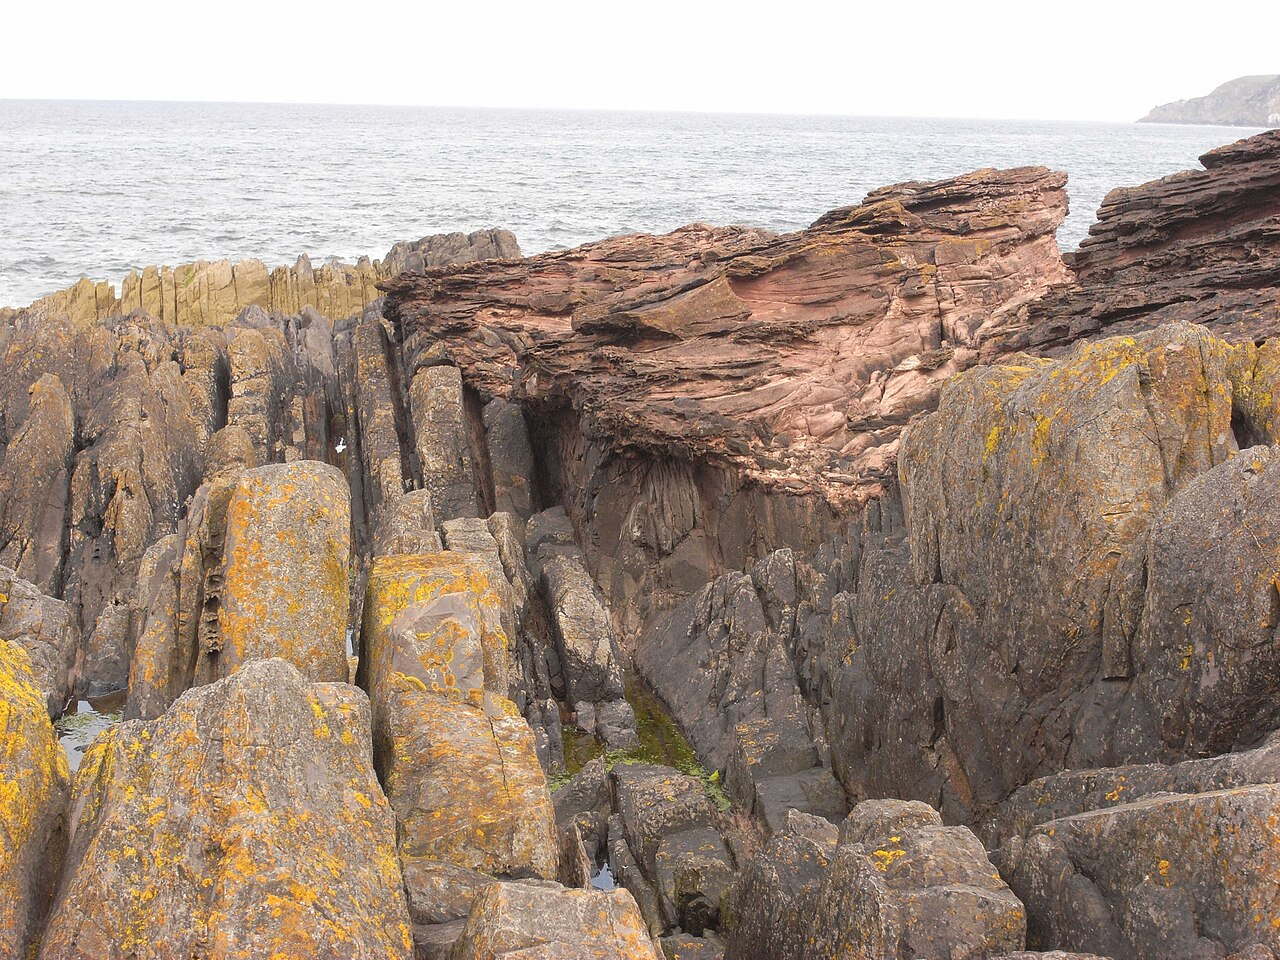
\includegraphics[width=.9\linewidth]{./Figs/Hutton_unconformity_siccar_point.jpg}
    \caption{Siccar Point}
    \label{fig:siccar_point__}
\end{figure}

A \textbf{discordância angular} ocorre quando estratos mais antigos foram inclinados, dobrados ou deformados e, após um intervalo de tempo acompanhado de erosão, passam a ser recobertos por camadas mais jovens depositadas em outra orientação. Nesse caso, o lapso temporal está associado não apenas à ausência de sedimentação contínua, mas também à atuação de processos tectônicos e erosivos entre os dois conjuntos de rochas.

\begin{figure}[H]
    \centering
    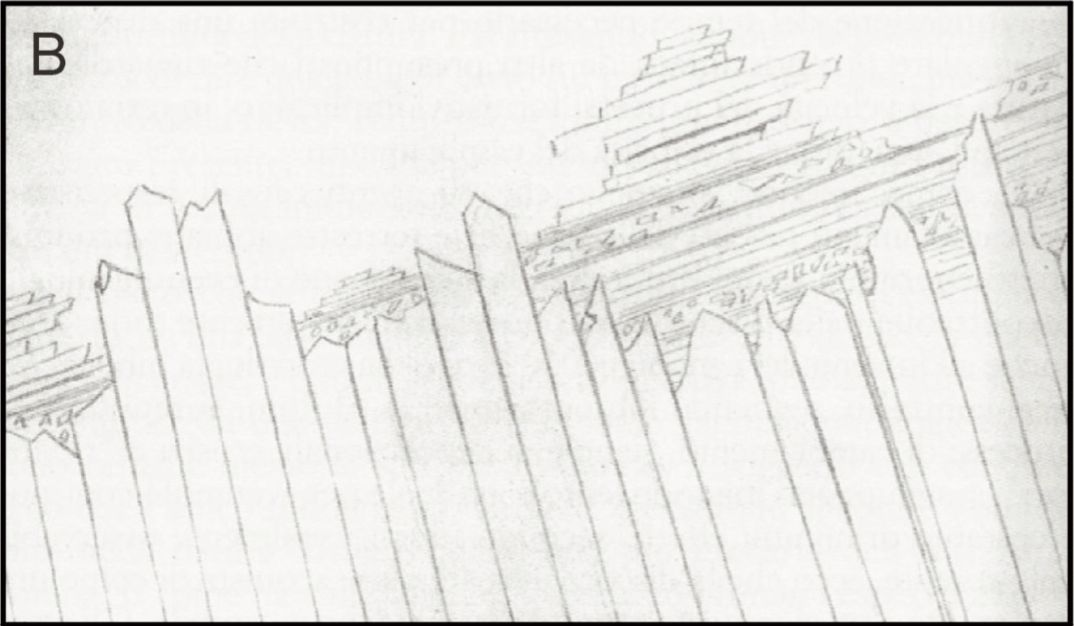
\includegraphics[width=.9\linewidth]{./Figs/Huttons_Unconformity_at_Sicar_Point_by_James_Hall_(1788).jpg}
    \caption{Siccar Point}
    \label{fig:siccar_point}
\end{figure}

A \textbf{desconformidade} ocorre entre camadas sedimentares aproximadamente paralelas, separadas por uma superfície erosiva ou por um hiato de não deposição. Embora a geometria entre os estratos não revele deformação evidente, existe ainda assim um intervalo de tempo ausente no registro, reconhecido pela erosão da superfície ou pela diferença de idade entre as unidades superpostas.

A \textbf{não conformidade} ocorre quando rochas sedimentares repousam diretamente sobre rochas ígneas ou metamórficas mais antigas. Nesse caso, o lapso temporal tende a ser particularmente expressivo, pois envolve a formação das rochas cristalinas em profundidade, sua exumação por soerguimento e erosão, e somente depois o estabelecimento de uma nova fase de sedimentação. Por isso, a não conformidade evidencia de forma especialmente clara a amplitude do tempo geológico envolvido na construção de uma paisagem e de seu registro rochoso.

\begin{figure}[H]
    \centering
    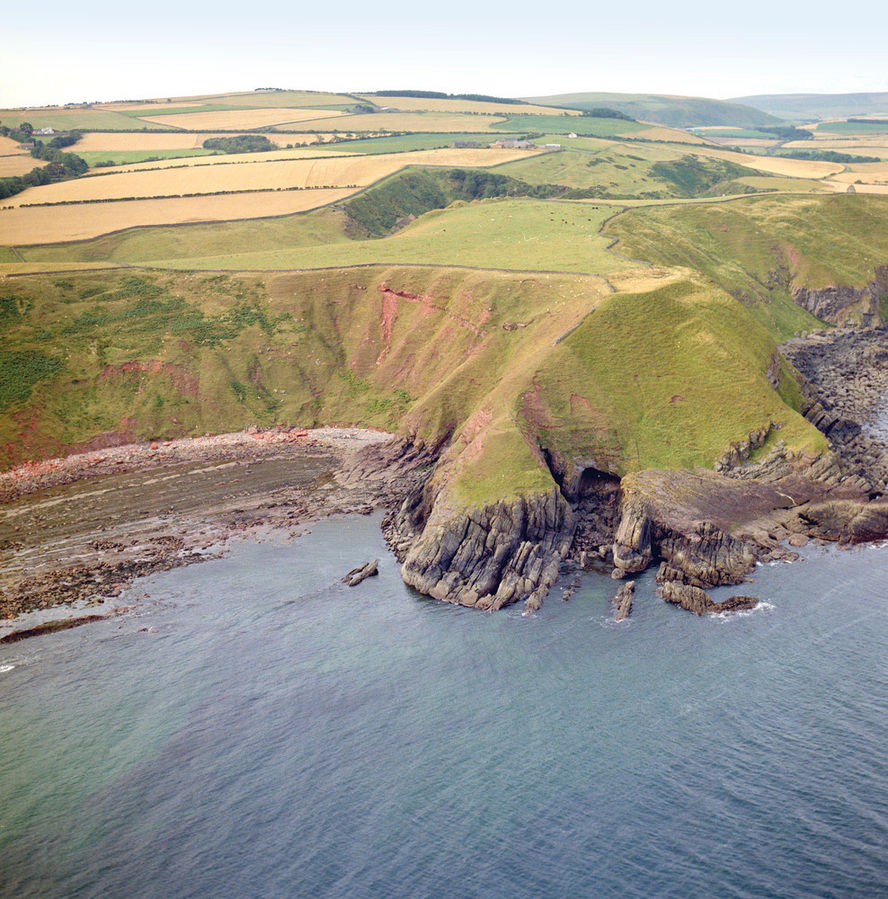
\includegraphics[width=0.9\linewidth]{Figs/afloramento.png}
    \caption{Discordância angular em Siccar Point, Escócia, local clássico associado a James Hutton, onde estratos mais antigos deformados e erodidos são recobertos por camadas sedimentares mais jovens. A feição ilustra a noção de hiato estratigráfico e sua relação com o tempo geológico profundo.}
    \label{fig:aflor}
\end{figure}


Assim, as discordâncias são fundamentais para a interpretação geológica, pois mostram que a história da Terra não é registrada apenas pelos estratos preservados, mas também pelos intervalos de tempo ausentes entre eles. Nesse sentido, a leitura proposta por Hutton foi decisiva ao demonstrar que uma superfície de discordância pode condensar uma longa sucessão de processos geológicos e, portanto, revelar a profundidade do tempo envolvido na evolução da crosta terrestre.

\section{Intemperismo}

\subsection{Definição}

O \textbf{intemperismo} é o conjunto de processos \textbf{físicos, químicos e biológicos} que provocam a \textbf{desagregação e/ou decomposição das rochas e dos minerais} quando estes ficam expostos às condições existentes na superfície ou próximo à superfície terrestre \parencite{boggs2012,tucker2001}.

As rochas que se formam em profundidade encontram condições de \textbf{pressão, temperatura e composição química} diferentes daquelas existentes na superfície. Quando essas rochas são expostas à atmosfera, à água, aos organismos e às variações de temperatura, muitos de seus minerais deixam de estar em equilíbrio com o novo ambiente e passam por transformações.

De forma geral, o intemperismo pode produzir:

\begin{itemize}
    \item fragmentos de rocha;
    \item grãos minerais;
    \item minerais secundários, como as argilas;
    \item íons dissolvidos na água;
    \item solos e mantos de alteração.
\end{itemize}

Portanto, o intemperismo constitui uma etapa fundamental do \textbf{ciclo das rochas} e também participa da formação dos \textbf{solos e dos sedimentos}, que posteriormente podem ser transportados e depositados.

É importante distinguir \textbf{intemperismo} de \textbf{erosão}:

\begin{itemize}
    \item \textbf{Intemperismo:} alteração ou desagregação da rocha \textbf{no próprio local};
    \item \textbf{Erosão:} remoção e transporte do material produzido pelo intemperismo.
\end{itemize}

Uma rocha pode, portanto, sofrer intemperismo sem que seus produtos sejam imediatamente transportados.

\subsection{Principais tipos de intemperismo}

Tradicionalmente, o intemperismo é dividido em três grandes grupos:

\begin{enumerate}
    \item \textbf{intemperismo físico ou mecânico};
    \item \textbf{intemperismo químico};
    \item \textbf{intemperismo biológico}.
\end{enumerate}

Na natureza, entretanto, esses processos normalmente atuam \textbf{simultaneamente} e podem intensificar uns aos outros.

\subsection{Intemperismo físico ou mecânico}

O \textbf{intemperismo físico} corresponde à fragmentação da rocha em pedaços menores \textbf{sem alteração significativa da composição química dos minerais}.

A rocha original é quebrada, mas os minerais que a formavam permanecem, inicialmente, com praticamente a mesma composição química.

Por exemplo, um bloco de granito pode ser dividido em fragmentos progressivamente menores, mas esses fragmentos ainda podem conter quartzo, feldspato e mica.

A principal consequência do intemperismo físico é o \textbf{aumento da área superficial da rocha}. Isso aumenta a superfície de contato entre os minerais e:

\begin{itemize}
    \item a água;
    \item o oxigênio;
    \item o dióxido de carbono;
    \item os organismos.
\end{itemize}

Consequentemente, o intemperismo físico pode acelerar o \textbf{intemperismo químico}.

\subsubsection{Alívio de pressão ou descompressão}

Muitas rochas se formam em grandes profundidades, submetidas a pressões elevadas devido ao peso das rochas que estão acima delas.

Quando a erosão remove progressivamente esse material superior, a pressão sobre a rocha diminui. Essa redução de pressão permite uma pequena expansão da rocha.

Como consequência, podem surgir \textbf{fraturas aproximadamente paralelas à superfície}, formando estruturas semelhantes a grandes lâminas ou cascas.

Esse processo é frequentemente chamado de \textbf{esfoliação por descompressão} e pode ser observado, por exemplo, em grandes corpos graníticos.

\subsubsection{Variação de temperatura}

As rochas podem sofrer aquecimento durante o dia e resfriamento durante a noite.

Quando aquecidos, os minerais tendem a se expandir; quando resfriados, tendem a se contrair.

Como diferentes minerais apresentam diferentes coeficientes de expansão térmica, ciclos repetidos de aquecimento e resfriamento podem gerar tensões dentro da rocha.

Ao longo de muitos ciclos, essas tensões podem contribuir para a formação e propagação de microfraturas.

Esse processo pode ser importante principalmente em ambientes submetidos a grandes variações térmicas. Entretanto, a simples variação diária de temperatura nem sempre é suficiente para explicar, isoladamente, uma intensa fragmentação das rochas, pois normalmente diversos mecanismos atuam simultaneamente.

\subsubsection{Congelamento da água em fraturas}

A água pode penetrar em pequenas fraturas existentes nas rochas.

Quando a temperatura cai abaixo do ponto de congelamento, essa água congela. A transformação da água líquida em gelo provoca aumento de volume.

Esse aumento exerce pressão sobre as paredes da fratura.

Quando ocorrem repetidos ciclos de

\[
\text{congelamento}
\rightarrow
\text{degelo}
\rightarrow
\text{congelamento},
\]

a fratura pode aumentar progressivamente até provocar a ruptura da rocha.

Esse mecanismo é particularmente importante em regiões frias e montanhosas sujeitas a frequentes ciclos de congelamento e degelo.

\subsubsection{Cristalização de sais}

Em ambientes onde existe água contendo sais dissolvidos, a água pode penetrar nos poros e fraturas das rochas.

Quando essa água evapora, os sais podem cristalizar.

O crescimento dos cristais dentro dos poros pode exercer pressão sobre os minerais e provocar a fragmentação da rocha.

Esse processo é chamado de \textbf{haloclastia} ou \textbf{intemperismo salino}.

Pode ser especialmente importante em:

\begin{itemize}
    \item ambientes costeiros;
    \item regiões áridas;
    \item áreas submetidas à névoa salina;
    \item rochas muito porosas.
\end{itemize}

Em regiões costeiras, os aerossóis marinhos podem introduzir sais nas superfícies rochosas, contribuindo para sua desagregação.

\subsubsection{Ação mecânica de organismos}

Raízes de plantas podem penetrar em pequenas fraturas.

Com o crescimento da raiz, aumenta a pressão exercida sobre as paredes da fratura, favorecendo a separação dos blocos.

Animais que escavam o solo também podem movimentar partículas, abrir canais e expor novos materiais à água e ao ar.

Nesse caso existe uma interação entre \textbf{intemperismo físico e biológico}.

\subsection{Intemperismo químico}

O \textbf{intemperismo químico} envolve reações que modificam a \textbf{composição química e/ou a estrutura mineralógica da rocha}.

Diferentemente do intemperismo físico, no qual ocorre principalmente fragmentação, no intemperismo químico alguns minerais originais podem ser:

\begin{itemize}
    \item dissolvidos;
    \item transformados;
    \item oxidados;
    \item hidratados;
    \item convertidos em novos minerais.
\end{itemize}

A água possui papel fundamental nesses processos.

Em muitos casos, a água funciona como:

\begin{itemize}
    \item solvente;
    \item meio onde ocorrem as reações;
    \item agente de transporte dos íons produzidos.
\end{itemize}

O intemperismo químico tende a ser particularmente intenso em regiões \textbf{quentes e úmidas}, pois temperaturas elevadas aumentam a velocidade de muitas reações químicas e a abundância de água favorece processos como dissolução e hidrólise.

\subsubsection{Dissolução}

A dissolução ocorre quando um mineral entra em contato com a água e seus componentes passam para a solução na forma de íons.

De maneira simplificada:

\[
\text{mineral sólido} + \text{água}
\rightarrow
\text{íons dissolvidos}
\]

Alguns minerais apresentam elevada solubilidade.

Um exemplo é a \textbf{halita}, formada por cloreto de sódio:

\[
\mathrm{NaCl_{(s)}
\rightarrow
Na^+_{(aq)} + Cl^-_{(aq)}}
\]

O mineral deixa de fazer parte da rocha e seus componentes passam para a água.

Esses íons podem posteriormente ser transportados por águas subterrâneas, rios e outros corpos d'água até alcançarem ambientes de deposição, incluindo os oceanos.

\subsubsection{Carbonatação}

A água da chuva contém dióxido de carbono dissolvido.

O dióxido de carbono reage com a água, formando ácido carbônico:

\[
\mathrm{CO_2 + H_2O
\rightleftharpoons
H_2CO_3}
\]

Embora seja um ácido relativamente fraco, o ácido carbônico aumenta a capacidade da água de reagir com determinados minerais.

Esse processo é especialmente importante em rochas carbonáticas, como os \textbf{calcários}.

A calcita, principal mineral de muitos calcários, pode reagir na presença de água e dióxido de carbono:

\[
\mathrm{CaCO_3 + CO_2 + H_2O
\rightarrow
Ca^{2+} + 2HCO_3^-}
\]

Esse processo favorece a dissolução do calcário.

Ao longo de grandes intervalos de tempo, pode contribuir para a formação de relevo cárstico, caracterizado por feições como:

\begin{itemize}
    \item cavernas;
    \item dolinas;
    \item condutos subterrâneos;
    \item sumidouros.
\end{itemize}

A precipitação posterior do carbonato de cálcio no interior de cavernas pode originar estruturas como estalactites e estalagmites.

\subsubsection{Hidrólise}

A \textbf{hidrólise} é um dos processos mais importantes do intemperismo químico dos \textbf{silicatos}, que constituem grande parte da crosta terrestre.

Nesse processo, minerais reagem com água, íons \(H^+\) e outras espécies presentes na solução.

Como resultado, minerais primários podem ser transformados em \textbf{minerais secundários}, especialmente argilominerais.

Um exemplo importante envolve os \textbf{feldspatos}.

De forma simplificada:

\[
\text{feldspato}
+
\text{água}
+
H^+
\rightarrow
\text{argilomineral}
+
\text{íons dissolvidos}
+
\text{sílica}
\]

Um exemplo balanceado é a alteração do feldspato potássico para caulinita:

\[
\mathrm{
2\,KAlSi_3O_8 + 2\,H_2CO_3 + 9\,H_2O
\rightarrow
Al_2Si_2O_5(OH)_4 + 4\,H_4SiO_4 + 2\,K^+ + 2\,HCO_3^-
}
\]

Nessa reação, a caulinita é um mineral secundário; potássio, bicarbonato e sílica dissolvida podem ser removidos pela água.

O feldspato existente originalmente numa rocha magmática pode, portanto, ser progressivamente transformado em minerais de argila.

Esse processo possui grande importância para a formação e evolução dos solos.

\subsubsection{Oxidação}

A \textbf{oxidação} envolve a perda de elétrons por determinados elementos químicos.

No intemperismo, um dos casos mais importantes envolve o \textbf{ferro}.

Minerais contendo ferro ferroso, \(Fe^{2+}\), podem sofrer oxidação, formando ferro férrico, \(Fe^{3+}\).

De maneira simplificada:

\[
Fe^{2+}
\rightarrow
Fe^{3+}
\]

Na presença de água e oxigênio podem ser formados óxidos e hidróxidos de ferro.

Esses produtos frequentemente apresentam cores:

\begin{itemize}
    \item avermelhadas;
    \item amareladas;
    \item alaranjadas;
    \item marrons.
\end{itemize}

Por isso, solos fortemente intemperizados em regiões tropicais frequentemente apresentam colorações avermelhadas ou amareladas.

\subsubsection{Hidratação}

Na \textbf{hidratação}, moléculas de água são incorporadas à estrutura de determinados minerais.

Essa incorporação pode provocar:

\begin{itemize}
    \item aumento de volume;
    \item alteração da estrutura mineral;
    \item redução da resistência do material.
\end{itemize}

Um exemplo é a transformação da anidrita em gipsita:

\[
\mathrm{CaSO_4 + 2H_2O
\rightarrow
CaSO_4\cdot 2H_2O}
\]

Nesse caso, a entrada de água modifica a estrutura cristalina do mineral.

\subsection{Intemperismo biológico}

O \textbf{intemperismo biológico} corresponde à participação dos seres vivos na alteração e desagregação das rochas.

Na prática, a atividade biológica pode provocar tanto efeitos físicos quanto químicos. Por isso, o intemperismo biológico não deve ser entendido como completamente separado dos demais tipos de intemperismo.

\subsubsection{Ação das raízes}

As raízes das plantas podem penetrar em fraturas existentes nas rochas.

À medida que crescem, exercem pressão mecânica, aumentando essas fraturas e favorecendo a fragmentação.

Ao mesmo tempo, raízes e microrganismos associados ao solo podem modificar quimicamente o ambiente.

\subsubsection{Produção de ácidos orgânicos}

A decomposição da matéria orgânica pode produzir diversos ácidos orgânicos.

Esses compostos podem:

\begin{itemize}
    \item reduzir o pH da água;
    \item aumentar a dissolução de minerais;
    \item facilitar a liberação de determinados elementos químicos.
\end{itemize}

Dessa maneira, os organismos podem acelerar o intemperismo químico.

\subsubsection{Líquens}

Os líquens são associações simbióticas que normalmente envolvem fungos e organismos fotossintetizantes.

Eles conseguem colonizar superfícies rochosas aparentemente pouco favoráveis à vida.

Sua presença pode favorecer a alteração das rochas principalmente pela retenção de umidade junto à superfície e pela produção de substâncias capazes de participar das reações químicas de alteração.

Ao longo do tempo, contribuem para a formação das primeiras camadas de material alterado sobre uma rocha exposta.

\subsection{Minerais e resistência ao intemperismo}

Nem todos os minerais apresentam a mesma resistência ao intemperismo.

Isso ocorre porque muitos minerais se formaram sob condições de temperatura e pressão muito diferentes das existentes na superfície terrestre.

De maneira geral, minerais formados em condições de temperatura mais elevada tendem a apresentar menor estabilidade química nas condições superficiais.

Minerais como:

\begin{itemize}
    \item olivina;
    \item piroxênio;
    \item anfibólio;
\end{itemize}

tendem a sofrer alteração química com relativa facilidade.

O \textbf{quartzo}, ao contrário, apresenta elevada resistência química nas condições superficiais.

Por isso, é extremamente comum encontrar grande quantidade de quartzo em:

\begin{itemize}
    \item areias;
    \item praias;
    \item dunas;
    \item depósitos sedimentares;
    \item solos.
\end{itemize}

Essa resistência ajuda a explicar por que muitas areias mineralogicamente maduras apresentam composição predominantemente quartzosa.

\subsubsection{Relação entre as séries de Bowen e Goldich}

A série de reação de Bowen descreve, de forma simplificada, a ordem de cristalização dos principais minerais silicáticos a partir de um magma em resfriamento.

\begin{figure}[H]
  \centering
  \resizebox{0.92\linewidth}{!}{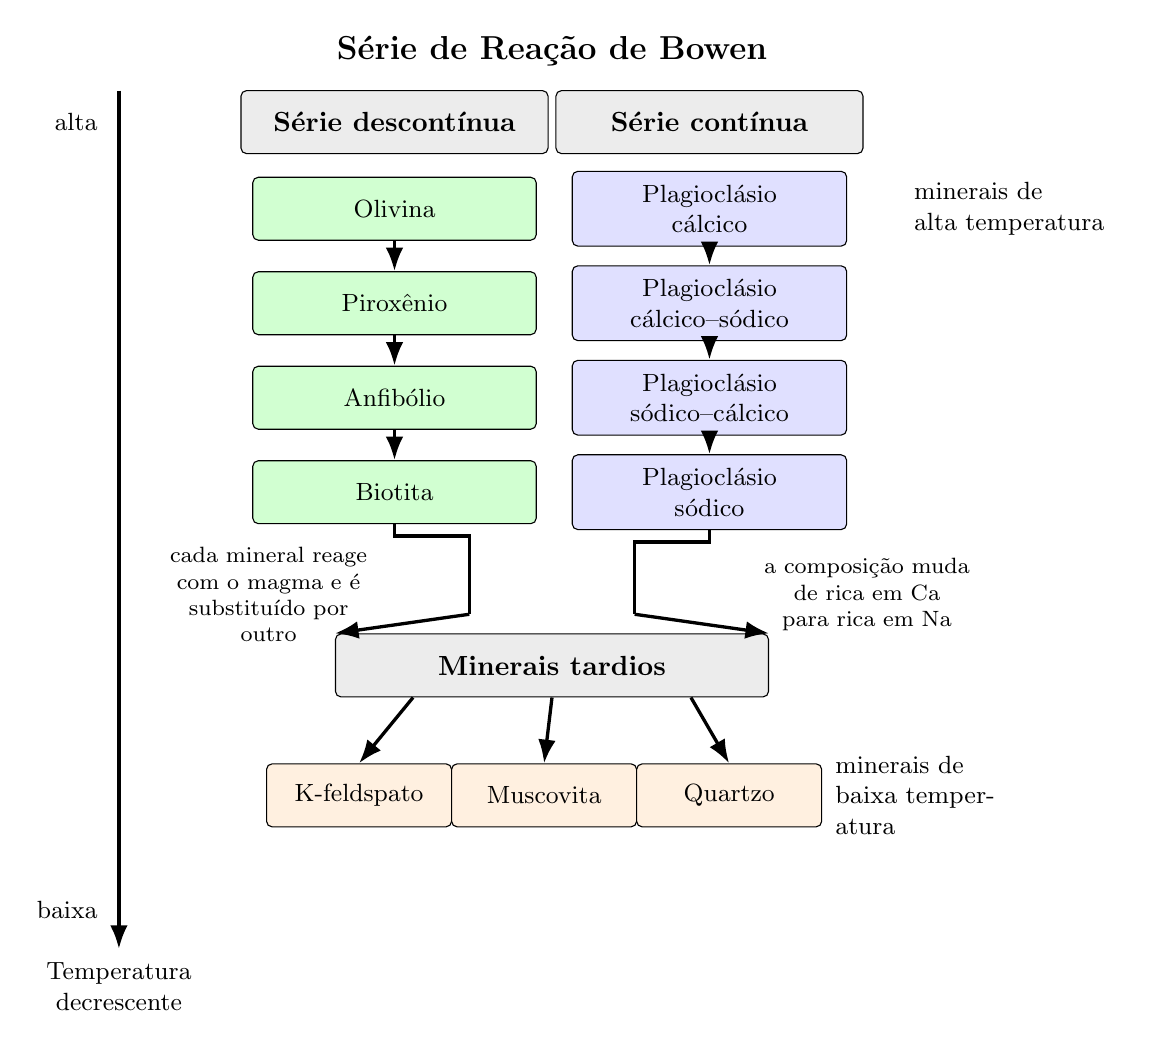
\begin{tikzpicture}[
    x=1cm,y=1cm,
    >=Latex,
    font=\small,
    titulo/.style={
        draw,
        rounded corners=2pt,
        fill=gray!15,
        font=\bfseries,
        minimum width=3.9cm,
        minimum height=0.8cm,
        align=center
    },
    mineralL/.style={
        draw,
        rounded corners=2pt,
        fill=green!18,
        minimum width=3.6cm,
        minimum height=0.8cm,
        align=center
    },
    mineralR/.style={
        draw,
        rounded corners=2pt,
        fill=blue!12,
        text width=3.25cm,
        minimum height=0.95cm,
        align=center
    },
    tardio/.style={
        draw,
        rounded corners=2pt,
        fill=orange!12,
        minimum width=2.35cm,
        minimum height=0.8cm,
        align=center
    },
    notaL/.style={
        align=center,
        text width=3.0cm,
        font=\footnotesize
    },
    notaR/.style={
        align=center,
        text width=3.3cm,
        font=\footnotesize
    }
]

% -------------------------------------------------
% Título geral
% -------------------------------------------------
\node[font=\bfseries\large] at (0.1,6.0) {Série de Reação de Bowen};

% -------------------------------------------------
% Eixo de temperatura
% -------------------------------------------------
\draw[very thick,-{Latex[length=3mm]}] (-5.4,5.5) -- (-5.4,-5.4);
\node[left] at (-5.55,5.1) {alta};
\node[left] at (-5.55,-4.9) {baixa};
\node[below,align=center] at (-5.4,-5.45) {Temperatura\\decrescente};

% -------------------------------------------------
% Cabeçalhos das colunas
% -------------------------------------------------
\node[titulo] (td) at (-1.9,5.1) {Série descontínua};
\node[titulo] (tc) at ( 2.1,5.1) {Série contínua};

% -------------------------------------------------
% Série descontínua
% -------------------------------------------------
\node[mineralL] (ol) at (-1.9,4.0) {Olivina};
\node[mineralL] (px) at (-1.9,2.8) {Piroxênio};
\node[mineralL] (am) at (-1.9,1.6) {Anfibólio};
\node[mineralL] (bt) at (-1.9,0.4) {Biotita};

\draw[very thick,-{Latex[length=3mm]}] (ol.south) -- (px.north);
\draw[very thick,-{Latex[length=3mm]}] (px.south) -- (am.north);
\draw[very thick,-{Latex[length=3mm]}] (am.south) -- (bt.north);

% -------------------------------------------------
% Série contínua
% -------------------------------------------------
\node[mineralR] (pl1) at (2.1,4.0) {Plagioclásio\\cálcico};
\node[mineralR] (pl2) at (2.1,2.8) {Plagioclásio\\cálcico--sódico};
\node[mineralR] (pl3) at (2.1,1.6) {Plagioclásio\\sódico--cálcico};
\node[mineralR] (pl4) at (2.1,0.4) {Plagioclásio\\sódico};

\draw[very thick,-{Latex[length=3mm]}] (pl1.south) -- (pl2.north);
\draw[very thick,-{Latex[length=3mm]}] (pl2.south) -- (pl3.north);
\draw[very thick,-{Latex[length=3mm]}] (pl3.south) -- (pl4.north);

% -------------------------------------------------
% Notas explicativas (deslocadas para não cruzar setas)
% -------------------------------------------------
\node[notaL] at (-3.5,-0.9)
{cada mineral reage com o magma e é \\substituído por \\outro};

\node[notaR] at (4.1,-0.9)
{a composição muda de rica em Ca\\para rica em Na};

% -------------------------------------------------
% Caixa central: minerais tardios
% -------------------------------------------------
\node[titulo, minimum width=5.5cm] (tf) at (0.1,-1.8) {Minerais tardios};

% -------------------------------------------------
% Conexões até a caixa central (desviadas do texto)
% -------------------------------------------------
\coordinate (ljoin) at (-0.95,-1.15);
\coordinate (rjoin) at ( 1.15,-1.15);

\draw[very thick]
    (bt.south) -- ++(0,-0.15) coordinate (btA)
    -- ++(0.95,0) coordinate (btB)
    -- (btB |- ljoin);
\draw[very thick,-{Latex[length=3mm]}]
    (btB |- ljoin) -- (tf.north west);

\draw[very thick]
    (pl4.south) -- ++(0,-0.15) coordinate (plA)
    -- ++(-0.95,0) coordinate (plB)
    -- (plB |- rjoin);
\draw[very thick,-{Latex[length=3mm]}]
    (plB |- rjoin) -- (tf.north east);

% -------------------------------------------------
% Minerais tardios finais
% -------------------------------------------------
\node[tardio] (kf) at (-2.35,-3.45) {K-feldspato};
\node[tardio] (ms) at ( 0.00,-3.45) {Muscovita};
\node[tardio] (qt) at ( 2.35,-3.45) {Quartzo};

% pontos de saída da caixa central
\coordinate (tfL) at ($(tf.south west)!0.18!(tf.south east)$);
\coordinate (tfC) at ($(tf.south west)!0.50!(tf.south east)$);
\coordinate (tfR) at ($(tf.south west)!0.82!(tf.south east)$);

\draw[very thick,-{Latex[length=3mm]}] (tfL) -- (kf.north);
\draw[very thick,-{Latex[length=3mm]}] (tfC) -- (ms.north);
\draw[very thick,-{Latex[length=3mm]}] (tfR) -- (qt.north);

% -------------------------------------------------
% Legendas laterais afastadas do desenho
% -------------------------------------------------
\node[align=left, text width=2.6cm] at (6.0,4.0)
{minerais de\\alta temperatura};

\node[align=left, text width=2.6cm] at (5.0,-3.45)
{minerais de\\baixa temperatura};

\end{tikzpicture}}
  \caption{Esquema simplificado da série de reação de Bowen.}
  \label{fig:bowen}
\end{figure}

Goldich observou que a suscetibilidade dos minerais ígneos ao intemperismo apresenta uma relação aproximadamente inversa com essa ordem de cristalização: minerais formados em temperaturas mais elevadas, como olivina e piroxênio, tendem a ser menos estáveis nas condições superficiais, enquanto o quartzo está entre os mais resistentes \parencite{goldich1938}. Essa relação é uma tendência geral, não uma regra absoluta, pois fraturamento, clima, pH, drenagem e tempo também controlam as taxas de alteração.

\subsection{Fatores que controlam o intemperismo}

A intensidade e o tipo de intemperismo dependem de diversos fatores, entre os quais se destacam:

\begin{itemize}
    \item clima;
    \item composição mineralógica;
    \item estrutura da rocha;
    \item relevo;
    \item presença de água;
    \item atividade biológica;
    \item tempo de exposição.
\end{itemize}

\subsubsection{Clima}

O clima é um dos fatores mais importantes no controle do intemperismo.

Em \textbf{climas quentes e úmidos}, existe elevada disponibilidade de água e as temperaturas mais altas favorecem a velocidade das reações químicas. Nessas condições, o intemperismo químico tende a ser intenso.

Em \textbf{climas frios}, processos associados aos ciclos de congelamento e degelo podem apresentar maior importância.

Em \textbf{climas áridos}, a menor disponibilidade de água limita muitas reações químicas. Entretanto, processos como cristalização de sais e variações térmicas podem apresentar maior importância relativa.

\subsubsection{Composição e estrutura da rocha}

A composição mineralógica determina em grande parte a resistência da rocha.

Uma rocha contendo minerais altamente resistentes pode permanecer exposta durante longo período sem sofrer intensa alteração química.

Por outro lado, minerais instáveis nas condições superficiais podem ser rapidamente transformados.

A estrutura e a textura da rocha também influenciam o intemperismo.

Uma rocha com muitas fraturas, elevada porosidade ou elevada permeabilidade permite maior penetração de água e maior superfície disponível para reações.

\subsubsection{Relevo}

A posição topográfica influencia a permanência dos materiais produzidos pelo intemperismo.

Em encostas muito inclinadas, os produtos de alteração podem ser removidos rapidamente pela gravidade e pela erosão.

Em terrenos de menor declividade, esses materiais podem permanecer por mais tempo sobre a rocha original, permitindo o desenvolvimento de mantos de alteração e solos mais espessos.

\subsubsection{Tempo}

O tempo também é fundamental para o desenvolvimento do intemperismo.

Quanto maior o período de exposição da rocha às condições superficiais, maior tende a ser seu grau de alteração, desde que existam condições adequadas para que os processos ocorram.

Entretanto, essa relação não é simplesmente linear, pois a formação de solos, a drenagem e a remoção dos produtos de alteração modificam continuamente as condições em que o intemperismo ocorre.

\subsection{Intemperismo e formação do solo}

O intemperismo é um dos processos fundamentais para a \textbf{pedogênese}, isto é, a formação e evolução dos solos.

A alteração das rochas produz:

\begin{itemize}
    \item fragmentos minerais;
    \item partículas finas;
    \item argilominerais;
    \item elementos químicos dissolvidos.
\end{itemize}

Esses materiais passam a interagir com matéria orgânica, organismos, água e atmosfera.

De maneira simplificada:

\[
\boxed{
\text{rocha}
\rightarrow
\text{intemperismo}
\rightarrow
\text{material alterado}
\rightarrow
\text{solo}
}
\]

\subsection{Intemperismo, erosão, transporte e sedimentação}

O intemperismo faz parte de uma sequência de processos fundamentais para a dinâmica superficial da Terra.

De maneira simplificada:

\[
\boxed{
\text{rocha}
\xrightarrow{\text{intemperismo}}
\text{material alterado}
\xrightarrow{\text{erosão}}
\text{transporte}
\xrightarrow{\text{deposição}}
\text{sedimento}
}
\]

Depois da deposição, os sedimentos podem sofrer processos de compactação, cimentação e outras transformações diagenéticas, podendo dar origem às \textbf{rochas sedimentares}.

\subsection{Intemperismo e sedimentos}

O intemperismo possui grande importância para a sedimentologia.

O intemperismo físico tende a produzir fragmentos progressivamente menores, enquanto o intemperismo químico pode destruir determinados minerais e formar novos minerais, como as argilas.

Por isso, um sedimento não representa necessariamente apenas pequenos fragmentos da rocha original.

Durante o intemperismo ocorre também uma espécie de \textbf{seleção mineralógica}.

Minerais menos resistentes tendem a ser:

\begin{itemize}
    \item dissolvidos;
    \item alterados;
    \item transformados em minerais secundários.
\end{itemize}

Minerais mais resistentes, como o quartzo, apresentam maior possibilidade de permanecer no sedimento.

Com sucessivos ciclos de

\[
\text{intemperismo}
+
\text{erosão}
+
\text{transporte}
+
\text{deposição},
\]

um sedimento pode tornar-se progressivamente mais \textbf{maduro mineralogicamente}.

\subsection{Intemperismo em ambientes costeiros}

Nos ambientes costeiros, diversos processos de intemperismo podem atuar simultaneamente.

Entre eles destacam-se:

\begin{itemize}
    \item ação da água;
    \item presença de sais;
    \item ciclos de umedecimento e secagem;
    \item atividade biológica;
    \item dissolução de minerais;
    \item oxidação;
    \item cristalização de sais.
\end{itemize}

A \textbf{haloclastia} pode ser especialmente relevante em superfícies rochosas submetidas à névoa e aos aerossóis marinhos.

A água contendo sais penetra nos poros e nas fraturas das rochas. Com a evaporação da água, pode ocorrer a cristalização dos sais.

Ciclos sucessivos de dissolução e cristalização podem favorecer a desagregação da superfície da rocha.

\subsection{Alteração esferoidal}

Um processo observado em algumas rochas é o chamado \textbf{intemperismo esferoidal} ou \textbf{alteração esferoidal}.

Quando um bloco rochoso fraturado sofre intemperismo químico, suas diferentes regiões não são alteradas com a mesma velocidade.

Os cantos apresentam maior superfície exposta em relação ao volume, seguidos pelas arestas e pelas faces.

De maneira simplificada:

\[
\text{cantos}
>
\text{arestas}
>
\text{faces}
\]

em relação à intensidade da alteração.

Com o tempo, blocos inicialmente angulosos podem adquirir formas progressivamente mais arredondadas.

É importante não confundir esse processo com o arredondamento provocado pelo transporte sedimentar.

No intemperismo esferoidal, o arredondamento ocorre \textbf{no próprio local}, como resultado da alteração diferencial da rocha.

\subsection{Perfil de intemperismo}

Quando o intemperismo atua durante longos períodos, pode desenvolver-se um \textbf{perfil de alteração} sobre a rocha.

De maneira simplificada, pode ocorrer a seguinte sequência vertical:

\[
\begin{array}{c}
\text{solo} \\[4pt]
\downarrow \\[4pt]
\text{material fortemente alterado} \\[4pt]
\downarrow \\[4pt]
\text{rocha parcialmente alterada} \\[4pt]
\downarrow \\[4pt]
\text{rocha sã}
\end{array}
\]

A transição entre essas zonas geralmente é gradual.

A espessura do perfil depende de fatores como:

\begin{itemize}
    \item clima;
    \item tempo;
    \item relevo;
    \item tipo de rocha;
    \item drenagem.
\end{itemize}

Em regiões tropicais úmidas, os perfis de alteração podem atingir grandes espessuras.

\subsection{Síntese}

Para fins didáticos, os três tipos principais de intemperismo podem ser resumidos da seguinte forma:

\paragraph{Intemperismo físico}

Produz principalmente a fragmentação da rocha:

\[
\text{rocha}
\rightarrow
\text{fragmentos menores}
\]

sem modificação química significativa dos minerais.

Entre seus principais mecanismos estão:

\begin{itemize}
    \item descompressão;
    \item congelamento e degelo;
    \item cristalização de sais;
    \item variações térmicas;
    \item ação mecânica de organismos.
\end{itemize}

\paragraph{Intemperismo químico}

Produz alterações na composição ou na estrutura dos minerais:

\[
\text{mineral original}
\rightarrow
\text{mineral secundário e/ou íons dissolvidos}
\]

Entre seus principais processos estão:

\begin{itemize}
    \item dissolução;
    \item hidrólise;
    \item carbonatação;
    \item oxidação;
    \item hidratação.
\end{itemize}

\paragraph{Intemperismo biológico}

Resulta da atividade dos organismos e pode provocar tanto efeitos físicos quanto efeitos químicos sobre as rochas.

\subsection{Importância geológica}

Uma maneira de compreender o intemperismo é considerar que uma rocha exposta na superfície terrestre encontra condições ambientais muito diferentes daquelas em que muitos de seus minerais originalmente se formaram.

Alguns minerais permanecem relativamente estáveis. Outros são alterados, dissolvidos ou transformados em novos minerais.

Ao mesmo tempo, a rocha pode ser progressivamente fraturada e desagregada.

O resultado conjunto desses processos fornece grande parte do material que posteriormente será submetido a:

\[
\boxed{
\text{erosão}
\rightarrow
\text{transporte}
\rightarrow
\text{deposição}
\rightarrow
\text{sedimentação}
}
\]

Por isso, o intemperismo constitui uma ligação fundamental entre a \textbf{geologia das rochas}, a \textbf{geomorfologia}, a \textbf{pedologia} e a \textbf{sedimentologia}, além de exercer importante influência sobre os processos que ocorrem nos ambientes continentais, costeiros e marinhos.


% =========================================================
% TRANSPORTE DE SEDIMENTOS
% =========================================================

\section{Transporte de Sedimentos}

\subsection{Definição}

O \textbf{transporte de sedimentos} corresponde ao deslocamento de partículas,
fragmentos de rocha, minerais e materiais biogênicos desde a área-fonte até os
locais onde serão posteriormente depositados. O transporte ocorre depois que o
material é produzido ou disponibilizado pelo intemperismo e pela erosão e
constitui uma etapa fundamental do ciclo sedimentar \parencite{nichols2009}.

De maneira simplificada:

\[
\boxed{
\text{intemperismo}
\rightarrow
\text{erosão}
\rightarrow
\text{transporte}
\rightarrow
\text{deposição}
\rightarrow
\text{sedimentação}
}
\]

Durante o transporte, os sedimentos podem sofrer modificações importantes, como:

\begin{itemize}
    \item fragmentação e abrasão;
    \item arredondamento dos grãos;
    \item seleção granulométrica;
    \item separação de minerais em função de densidade, tamanho e resistência;
    \item retrabalhamento sucessivo.
\end{itemize}

Assim, as características de um depósito sedimentar refletem não apenas a
natureza da rocha-fonte, mas também os agentes, a distância, a duração e a
energia envolvida no transporte.

\subsection{Principais agentes de transporte}

Os principais agentes capazes de transportar sedimentos são:

\begin{enumerate}
    \item água;
    \item vento;
    \item gelo;
    \item gravidade.
\end{enumerate}

A água constitui um dos principais agentes de transporte, especialmente nos
sistemas fluviais, lacustres, estuarinos, deltaicos, costeiros e marinhos.

\subsection{Modos de transporte sedimentar}

Os principais modos de transporte são:

\begin{itemize}
    \item tração;
    \item saltação;
    \item suspensão;
    \item transporte em solução.
\end{itemize}

Um mesmo grão pode mudar de modo de transporte quando variam a velocidade, a
turbulência e a energia do fluxo.

\subsubsection{Tração}

A \textbf{tração} corresponde ao transporte de partículas junto ao fundo. Os
grãos podem deslocar-se por rolamento, deslizamento ou arraste.

Esse mecanismo é importante para partículas relativamente grossas ou pesadas,
como areia grossa, grânulos, seixos e cascalhos. Para que o movimento se inicie,
a força exercida pelo fluido deve superar a resistência associada ao peso do
grão, ao atrito com o fundo e ao encaixe entre as partículas.

\subsubsection{Saltação}

Na \textbf{saltação}, as partículas deslocam-se por uma sequência de pequenos
saltos sobre o substrato. O fluxo eleva temporariamente o grão, que percorre uma
determinada distância e retorna ao fundo.

De maneira esquemática:

\[
\text{repouso}
\rightarrow
\text{elevação}
\rightarrow
\text{deslocamento}
\rightarrow
\text{impacto}
\rightarrow
\text{novo salto}
\]

A saltação é especialmente importante no transporte de areia e ocorre tanto em
ambientes subaquosos quanto eólicos. Esse mecanismo participa da formação e da
migração de marcas onduladas e dunas.

\subsubsection{Suspensão}

Na \textbf{suspensão}, as partículas permanecem temporariamente mantidas dentro
da coluna de fluido, principalmente pela turbulência.

Esse mecanismo é especialmente importante para materiais finos, como:

\begin{itemize}
    \item argila;
    \item silte;
    \item areia muito fina.
\end{itemize}

Quanto menor a velocidade de queda da partícula, maior sua tendência a
permanecer em suspensão. Por essa razão, sedimentos muito finos podem ser
transportados por grandes distâncias.

\subsubsection{Transporte em solução}

Parte dos produtos do intemperismo químico é transportada na forma de íons
dissolvidos. Entre os principais componentes transportados em solução estão:

\[
Ca^{2+}, \quad Na^+, \quad K^+, \quad Mg^{2+}
\]

e

\[
HCO_3^-, \quad Cl^-, \quad SO_4^{2-}.
\]

Alterações posteriores das condições físico-químicas da água podem provocar a
precipitação desses componentes, contribuindo para a formação de sedimentos
químicos.

\subsection{Carga sedimentar}

Em sistemas fluviais, a carga transportada pode ser dividida em três componentes
principais.

\subsubsection{Carga de fundo}

A \textbf{carga de fundo} é formada pelo material que permanece próximo ou em
contato frequente com o leito e é transportado principalmente por tração e
saltação.

\subsubsection{Carga em suspensão}

A \textbf{carga em suspensão} corresponde às partículas mantidas na coluna
d'água pela turbulência, principalmente silte, argila e parte da areia fina.

\subsubsection{Carga dissolvida}

A \textbf{carga dissolvida} é constituída por íons e moléculas transportados em
solução.

\subsection{Competência e capacidade de transporte}

Dois conceitos importantes para compreender o comportamento de um fluxo são
\textbf{competência} e \textbf{capacidade}.

A \textbf{competência} corresponde ao maior tamanho de partícula que um fluxo
consegue transportar. Assim, de maneira geral:

\[
\text{maior energia do fluxo}
\Rightarrow
\text{maior competência}
\]

A \textbf{capacidade}, por sua vez, corresponde à quantidade total de sedimento
que o fluxo consegue transportar.

Portanto:

\begin{itemize}
    \item competência relaciona-se principalmente ao tamanho máximo dos grãos;
    \item capacidade relaciona-se principalmente à quantidade total de sedimento.
\end{itemize}

\subsection{Velocidade do fluxo e granulometria}

A erosão, o transporte e a deposição dependem da interação entre:

\begin{itemize}
    \item velocidade do fluxo;
    \item turbulência;
    \item tamanho e densidade dos grãos;
    \item forma das partículas;
    \item viscosidade e densidade do fluido;
    \item coesão do sedimento;
    \item características do fundo.
\end{itemize}

Correntes mais energéticas podem transportar partículas maiores. Entretanto, a
relação entre tamanho do grão e facilidade de erosão não é linear. Partículas
argilosas, apesar de muito pequenas, podem exigir velocidades relativamente
elevadas para serem erodidas devido às forças de coesão entre os grãos.

Assim:

\[
\text{grão pequeno}
\not\Rightarrow
\text{necessariamente fácil erosão}.
\]

\subsection{Número de Froude e regimes de fluxo}

Em canais abertos, o número de Froude compara a velocidade média do fluxo com a velocidade de propagação de ondas gravitacionais rasas:

\[
\mathrm{Fr}=\frac{U}{\sqrt{gD}},
\]

em que \(U\) é a velocidade média, \(g\) é a aceleração da gravidade e \(D\) é uma profundidade característica do fluxo.

\begin{itemize}
  \item \(\mathrm{Fr}<1\): fluxo \textbf{subcrítico}, no qual perturbações podem se propagar para montante;
  \item \(\mathrm{Fr}=1\): condição \textbf{crítica};
  \item \(\mathrm{Fr}>1\): fluxo \textbf{supercrítico}, no qual a velocidade do fluxo supera a das ondas rasas.
\end{itemize}

Em leitos arenosos, o regime inferior inclui comumente ripples, dunas e leito plano inferior. Com o aumento da velocidade e do transporte em suspensão, podem surgir leito plano superior, antidunas e outras formas relacionadas ao regime superior. A forma efetivamente produzida depende também da granulometria, da profundidade e da carga sedimentar \parencite{harms1975,nichols2009}.

\subsection{Diagrama de Hjulström}

A relação entre tamanho das partículas e velocidade da corrente é
tradicionalmente representada pelo \textbf{diagrama de Hjulström}. O diagrama
distingue três campos principais:

\begin{enumerate}
    \item erosão;
    \item transporte;
    \item deposição.
\end{enumerate}

As areias apresentam valores relativamente baixos de velocidade crítica para o
início do movimento. As argilas, apesar de muito finas, podem exigir velocidades
mais elevadas para serem erodidas devido à coesão. Uma vez colocadas em
suspensão, entretanto, podem continuar sendo transportadas mesmo quando a
velocidade do fluxo diminui.

\subsection{Velocidade de queda}

A \textbf{velocidade de queda} corresponde à velocidade com que uma partícula
tende a se deslocar em direção ao fundo sob a ação da gravidade.

Ela depende de fatores como:

\begin{itemize}
    \item tamanho;
    \item densidade;
    \item forma da partícula;
    \item densidade do fluido;
    \item viscosidade do fluido.
\end{itemize}

De forma geral:

\[
\text{partículas maiores e mais densas}
\Rightarrow
\text{maior velocidade de queda}.
\]

Quando a energia de um fluxo diminui, as partículas maiores normalmente tendem
a ser depositadas antes das menores.

\subsection{Seleção granulométrica}

Durante o transporte pode ocorrer \textbf{seleção granulométrica}, pois partículas
de diferentes tamanhos e densidades respondem de maneiras distintas ao mesmo
fluxo.

Um sedimento é considerado:

\begin{itemize}
    \item \textbf{bem selecionado}, quando apresenta pequena variação granulométrica;
    \item \textbf{mal selecionado}, quando apresenta ampla variação dos tamanhos dos grãos.
\end{itemize}

O vento e correntes persistentes podem produzir depósitos relativamente bem
selecionados. Geleiras e determinados fluxos gravitacionais, por outro lado,
podem produzir depósitos muito mal selecionados.

\subsection{Abrasão, arredondamento e maturidade}

Durante o transporte, os grãos podem colidir entre si, com o fundo e com
obstáculos presentes no percurso. Essas colisões provocam \textbf{abrasão}, com
desgaste progressivo de cantos e arestas.

De maneira geral:

\[
\text{maior retrabalhamento}
\Rightarrow
\text{maior tendência ao arredondamento}.
\]

O grau de arredondamento também depende da mineralogia, da dureza, do tamanho do
grão e do mecanismo de transporte.

O retrabalhamento sucessivo pode aumentar a maturidade do sedimento. A
\textbf{maturidade textural} relaciona-se principalmente ao grau de seleção, ao
arredondamento dos grãos e à quantidade de matriz fina. A
\textbf{maturidade mineralógica} relaciona-se à proporção de minerais
resistentes. Minerais pouco estáveis tendem a ser alterados ou destruídos,
enquanto minerais resistentes, como o quartzo, podem tornar-se
proporcionalmente mais abundantes.

\subsection{Transporte pelo vento}

O vento atua principalmente sobre sedimentos secos e pouco coesivos. O
transporte eólico ocorre sobretudo por saltação, suspensão e arraste superficial.

Como o ar possui densidade muito menor que a água, sua competência para
transportar partículas grossas é relativamente limitada. Os depósitos eólicos
são geralmente dominados por areia e silte e podem apresentar boa seleção
granulométrica.

\subsection{Transporte pelo gelo}

As geleiras são capazes de transportar sedimentos com ampla variação
granulométrica, desde argila e silte até grandes blocos de rocha.

O transporte glacial apresenta baixa eficiência de seleção, podendo produzir
depósitos constituídos por partículas de tamanhos muito diferentes.

\subsection{Transporte por gravidade}

A gravidade pode produzir deslocamento de sedimentos ao longo das encostas por
processos como:

\begin{itemize}
    \item queda de blocos;
    \item escorregamentos;
    \item deslizamentos;
    \item fluxos de detritos;
    \item fluxos de lama.
\end{itemize}

Os depósitos resultantes frequentemente apresentam baixa seleção e podem conter
clastos relativamente angulosos.

\subsection{Fluxos gravitacionais subaquosos}

Em ambientes submarinos também podem ocorrer movimentos gravitacionais de
sedimentos. Entre os mais importantes estão as \textbf{correntes de turbidez},
formadas por misturas de água e sedimentos com densidade maior que a água
circundante.

À medida que o fluxo perde energia, as partículas maiores tendem a se depositar
antes das menores, podendo produzir uma gradação normal:

\[
\text{base mais grossa}
\rightarrow
\text{topo mais fino}.
\]

Os depósitos produzidos por correntes de turbidez são chamados de
\textbf{turbiditos}.

\subsection{Transporte em ambientes costeiros}

Nos ambientes costeiros, o transporte sedimentar resulta da interação entre:

\begin{itemize}
    \item ondas;
    \item correntes;
    \item marés;
    \item descargas fluviais;
    \item vento.
\end{itemize}

As ondas podem colocar partículas do fundo em movimento ou suspensão, enquanto
as correntes promovem seu deslocamento. O transporte longitudinal ao longo da
costa exerce importante papel na evolução de praias, pontais e demais feições
sedimentares costeiras.

\subsection{Floculação das argilas}

As partículas de argila apresentam dimensões muito pequenas e podem permanecer
em suspensão por longos períodos. Em ambientes estuarinos, a mistura entre água
doce e água salgada pode favorecer a agregação das partículas finas.

Esse processo é denominado \textbf{floculação}. Os agregados, ou flocos,
apresentam velocidade de queda maior do que as partículas individuais,
favorecendo a deposição de sedimentos finos.

\subsection{Relação entre transporte e deposição}

A deposição ocorre quando o agente de transporte deixa de possuir energia
suficiente para manter determinada partícula em movimento.

De maneira simplificada, quando a energia diminui progressivamente, tende a
ocorrer a seguinte sequência de deposição:

\[
\text{cascalho}
\rightarrow
\text{areia}
\rightarrow
\text{silte}
\rightarrow
\text{argila}.
\]

Essa sequência é uma simplificação, pois coesão, floculação, turbulência e
características específicas do fluxo também influenciam a deposição.


% =========================================================
% ESTRUTURAS SEDIMENTARES
% =========================================================

\section{Deposição, sedimentação e bacias sedimentares}

\begin{definicao}
\textbf{Deposição} é a retirada de partículas ou substâncias do meio transportador e seu acúmulo em determinado local. \textbf{Sedimentação} é o processo mais amplo de formação e acumulação de sedimentos, incluindo componentes detríticos, químicos e biogênicos.
\end{definicao}

A deposição de partículas ocorre quando o agente transportador perde competência ou capacidade, quando há mudança na geometria do fluxo ou quando as partículas encontram uma barreira. Substâncias dissolvidas podem precipitar em resposta a evaporação, mudanças de temperatura, pH, estado de oxidação ou atividade biológica.

\subsection{Espaço de acomodação}

O \textbf{espaço de acomodação} é o volume disponível para que sedimentos se acumulem e sejam preservados. Ele pode ser produzido por subsidência tectônica, variação do nível de base, compactação ou mudanças na topografia. Quando a taxa de criação de acomodação e o suprimento sedimentar variam, modificam-se a geometria e o empilhamento dos depósitos.

\subsection{Bacia de sedimentação e bacia sedimentar}

Uma \textbf{bacia de sedimentação} é uma área em que ocorre acumulação de sedimentos. Uma \textbf{bacia sedimentar} é uma região subsidente da crosta que recebeu e preservou um preenchimento sedimentar ao longo do tempo geológico. Portanto, nem todo local de deposição temporária constitui, no sentido tectonoestratigráfico, uma bacia sedimentar.

\begin{figure}[H]
  \centering
  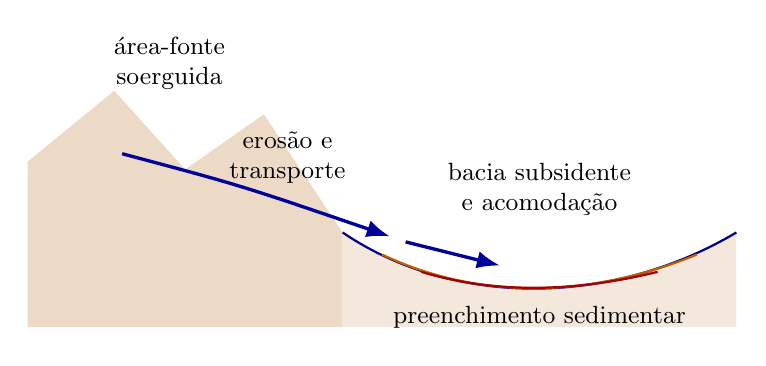
\begin{tikzpicture}[x=1cm,y=1cm,>=Latex,font=\small]
    \fill[brown!30] (0,0) -- (0,2.1) -- (1.1,3.0) -- (2.0,2.0)
      -- (3.0,2.7) -- (4.0,1.2) -- (4.0,0) -- cycle;
    \fill[brown!18] (4,0) -- (4,1.2)
      .. controls (5.4,0.25) and (7.4,0.25) .. (9,1.2)
      -- (9,0) -- cycle;
    \draw[blue!55!black,thick]
      (4,1.2) .. controls (5.4,0.25) and (7.4,0.25) .. (9,1.2);
    \draw[orange!75!black,thick]
      (4.5,0.92) .. controls (5.7,0.35) and (7.1,0.35) .. (8.5,0.92);
    \draw[red!65!black,thick]
      (5.0,0.70) .. controls (5.9,0.43) and (6.9,0.43) .. (8.0,0.70);
    \draw[->,very thick,blue!60!black] (1.2,2.2) .. controls (2.7,1.8) .. (4.6,1.15);
    \draw[->,very thick,blue!60!black] (4.8,1.08) -- (6.0,0.78);
    \node[align=center] at (1.8,3.35) {área-fonte\\soerguida};
    \node[align=center] at (3.3,2.15) {erosão e\\transporte};
    \node[align=center] at (6.5,1.75) {bacia subsidente\\e acomodação};
    \node[align=center] at (6.5,0.12) {preenchimento sedimentar};
  \end{tikzpicture}
  \caption{Relação simplificada entre área-fonte, transporte, subsidência e preenchimento de uma bacia.}
  \label{fig:bacia-sedimentar}
  \caption*{\footnotesize Fonte: elaborado pelo autor com base em \textcite{nichols2009}.}
\end{figure}

\subsection{Soerguimento e subsidência}

O \textbf{soerguimento} favorece a exposição de rochas, o desenvolvimento do relevo e a erosão da área-fonte. A \textbf{subsidência} cria ou amplia espaço de acomodação e pode favorecer a preservação dos depósitos. Os dois processos podem ocorrer em regiões distintas de um mesmo sistema sedimentar e variar ao longo do tempo.

\subsection{Produtos da sedimentação}

Uma bacia pode receber sedimentos siliciclásticos e vulcanoclásticos, produzir carbonatos e matéria orgânica ou registrar precipitação química. Evaporitos incluem, entre outros, sulfatos, como gipsita e anidrita, e cloretos, como halita. Carvões, depósitos silicosos e formações ferríferas representam outros produtos sedimentares que dependem de condições ambientais e geoquímicas específicas \parencite{nichols2009}.

\section{Granulometria, textura e morfologia dos grãos}

\begin{definicao}
\textbf{Granulometria} é a descrição da distribuição dos tamanhos das partículas de um sedimento ou rocha sedimentar. Ela pode ser determinada por peneiramento, sedimentação, difração a laser ou análise de imagens, conforme a faixa de tamanhos e o objetivo do estudo.
\end{definicao}

\subsection{Escala de Udden--Wentworth}

A escala de Udden--Wentworth organiza os sedimentos clásticos em classes cujos limites variam por fatores de dois \parencite{wentworth1922}. Os limites fundamentais são:

\begin{table}[H]
  \centering
  \caption{Classes granulométricas fundamentais.}
  \label{tab:wentworth-resumo}
  \begin{tabular}{lll}
    \toprule
    \textbf{Fração} & \textbf{Diâmetro aproximado} & \textbf{Rocha consolidada} \\
    \midrule
    Cascalho & maior que \SI{2}{\milli\metre} & conglomerado ou brecha \\
    Areia    & \SIrange{0.0625}{2}{\milli\metre} & arenito \\
    Silte    & \SIrange{0.0039}{0.0625}{\milli\metre} & siltito \\
    Argila   & menor que \SI{0.0039}{\milli\metre} & argilito \\
    \bottomrule
  \end{tabular}
\end{table}

Na escala phi, usada em sedimentologia, o tamanho é expresso por

\[
\phi=-\log_2 d,
\]

em que \(d\) é o diâmetro da partícula em milímetros. Assim, valores maiores de \(\phi\) representam partículas menores.

\subsection{Seleção granulométrica}

A \textbf{seleção} indica a dispersão dos tamanhos dos grãos. Um sedimento bem selecionado concentra-se em poucas classes granulométricas; um sedimento mal selecionado contém ampla variedade de tamanhos. A seleção depende do agente, da energia e da duração do transporte, mas também pode ser herdada da área-fonte.

Quando a distribuição é quantificada em unidades phi, podem ser empregadas classes como muito bem selecionada, bem selecionada, moderadamente selecionada, mal selecionada e muito mal selecionada. O método estatístico e os limites adotados devem ser declarados, pois classificações distintas coexistem na literatura.

\subsection{Arredondamento e esfericidade}

\textbf{Arredondamento} e \textbf{esfericidade} descrevem propriedades diferentes:

\begin{itemize}
  \item o \textbf{arredondamento} avalia a curvatura das arestas e dos vértices;
  \item a \textbf{esfericidade} avalia quanto a forma geral do grão se aproxima de uma esfera.
\end{itemize}

Um grão pode, portanto, ser bem arredondado e apresentar baixa esfericidade. A escala visual de Powers distingue seis classes de arredondamento: muito angular, angular, subangular, subarredondado, arredondado e bem arredondado \parencite{powers1953}.

\subsection{Arcabouço, matriz, cimento e poros}

Na descrição textural de uma rocha siliciclástica devem ser reconhecidos:

\begin{itemize}
  \item \textbf{arcabouço}: conjunto dos grãos que formam a estrutura principal;
  \item \textbf{matriz}: material detrítico mais fino depositado entre os grãos;
  \item \textbf{cimento}: mineral precipitado durante a diagênese;
  \item \textbf{poros}: espaços vazios que podem armazenar fluidos.
\end{itemize}

Matriz e cimento não são sinônimos: a matriz é deposicional ou sinsedimentar, enquanto o cimento se forma por precipitação diagenética.

\subsection{Exemplo de descrição textural}

Uma amostra composta por aproximadamente 80\% de areia fina, 10\% de areia média e 10\% de grânulos apresenta predomínio de areia fina, mas contém uma fração grossa relevante. A presença simultânea dessas classes sugere seleção baixa a moderada. A descrição deve ser completada com arredondamento, esfericidade, tipo de suporte, proporção de matriz e composição mineralógica, por exemplo, predomínio de quartzo e feldspato.

\section{Estruturas Sedimentares}

\subsection{Definição}

As \textbf{estruturas sedimentares} são feições desenvolvidas durante ou após a
deposição dos sedimentos e que podem permanecer preservadas no depósito ou na
rocha resultante de sua litificação \parencite{harms1975,nichols2009}.

Essas estruturas constituem registros dos processos responsáveis pela formação
do depósito e permitem interpretar aspectos como:

\begin{itemize}
    \item direção e sentido das paleocorrentes;
    \item regime e energia do fluxo;
    \item mecanismos de transporte e deposição;
    \item exposição subaérea;
    \item processos químicos ocorridos durante ou após a deposição;
    \item presença e atividade de organismos;
    \item deformação de sedimentos ainda inconsolidados.
\end{itemize}

De acordo com sua origem, podem ser agrupadas em:

\begin{enumerate}
    \item estruturas físicas ou mecânicas;
    \item estruturas químicas;
    \item estruturas biogênicas.
\end{enumerate}

\subsection{Estruturas físicas ou mecânicas}

As \textbf{estruturas físicas} resultam principalmente da ação mecânica dos
agentes de transporte, deposição ou deformação dos sedimentos, como correntes,
ondas, marés, vento e gravidade.

\subsubsection{Estratificação}

A \textbf{estratificação} corresponde à organização dos sedimentos em camadas ou
estratos. Cada estrato pode representar um episódio de deposição ou um intervalo
durante o qual determinadas condições sedimentares permaneceram relativamente
constantes.

As superfícies que separam os estratos são denominadas
\textbf{planos de estratificação}. Mudanças entre camadas podem refletir
variações de granulometria, composição, cor, energia do ambiente e velocidade de
sedimentação.

\subsubsection{Laminação}

A \textbf{laminação} corresponde à organização do sedimento em camadas muito
delgadas. As lâminas podem resultar de pequenas variações de granulometria,
composição ou condições de fluxo.

Quando apresentam geometria aproximadamente horizontal e paralela, constituem a
\textbf{laminação plano-paralela}.

\subsubsection{Estratificação cruzada}

A \textbf{estratificação cruzada} ocorre quando conjuntos de lâminas encontram-se
inclinados em relação ao plano principal de estratificação.

Sua formação está normalmente associada à migração de formas de leito, como
marcas onduladas, dunas subaquosas, dunas eólicas e barras. A orientação das
lâminas pode fornecer informações sobre a direção do paleofluxo.

Em ambientes com reversão periódica de corrente, conjuntos inclinados em sentidos opostos podem formar \textbf{estratificação cruzada espinha de peixe}. Superfícies de reativação registram erosão parcial e retomada da migração de uma forma de leito, frequentemente após mudança na intensidade ou na direção do fluxo.

\subsubsection{Marcas onduladas}

As \textbf{marcas onduladas}, ou \textit{ripple marks}, são pequenas ondulações
formadas na superfície de sedimentos inconsolidados pela ação da água ou do
vento.

As marcas produzidas por corrente são normalmente assimétricas e podem indicar o
sentido predominante do fluxo. As produzidas pela ação oscilatória das ondas
tendem a apresentar maior simetria.

\subsubsection{Acamamentos flaser, ondulado e lenticular}

Quando areia e lama se alternam sob variações periódicas da energia, podem formar-se três padrões principais:

\begin{itemize}
  \item \textbf{flaser}: lâminas descontínuas de lama preservadas entre ripples predominantemente arenosos;
  \item \textbf{ondulado} (\textit{wavy}): proporções semelhantes de areia e lama formam camadas lateralmente contínuas e onduladas;
  \item \textbf{lenticular}: lentes isoladas de areia ficam envolvidas por lama.
\end{itemize}

Esses padrões são comuns em depósitos submetidos à alternância entre correntes capazes de transportar areia e períodos de baixa energia que permitem a decantação de lama \parencite{nichols2009}.

\subsubsection{Estratificação cruzada hummocky e swaley}

A estratificação cruzada \textit{hummocky} apresenta laminações suavemente curvas, com elevações e depressões de baixo ângulo. É associada principalmente a fluxos combinados produzidos por ondas e correntes durante tempestades em ambientes marinhos rasos. A variante \textit{swaley} é dominada por depressões erosivas e tende a ocorrer em condições de maior retrabalhamento. A interpretação deve considerar a associação de fácies e não apenas uma geometria isolada \parencite{harms1975,nichols2009}.

\subsubsection{Estratificação gradacional}

A \textbf{estratificação gradacional} ocorre quando há variação sistemática do
tamanho dos grãos ao longo de uma camada.

Na gradação normal:

\[
\text{base grossa}
\rightarrow
\text{topo fino}.
\]

Esse padrão geralmente indica diminuição progressiva da energia do fluxo durante
a deposição. Também pode ocorrer gradação inversa, na qual o tamanho dos grãos
aumenta em direção ao topo.

\subsubsection{Marcas de sola}

As \textbf{marcas de sola} são feições preservadas principalmente na base de
camadas sedimentares. Podem ser formadas quando correntes erodem um substrato
ainda inconsolidado e as depressões resultantes são posteriormente preenchidas
por sedimento.

Algumas dessas estruturas permitem interpretar direção e sentido de
paleocorrentes.

\subsubsection{Gretas de dessecação}

As \textbf{gretas de dessecação} formam-se quando sedimentos finos, úmidos e
coesivos são expostos ao ar e perdem água. A retração do material produz uma rede
de fraturas frequentemente poligonais.

Sua presença indica exposição subaérea temporária e pode ocorrer em planícies de
maré, margens de lagos, planícies de inundação e outras áreas sujeitas a
alternância entre inundação e secagem.

\subsubsection{Estruturas de carga e deformações sinsedimentares}

As \textbf{estruturas de carga} podem desenvolver-se quando uma camada mais densa
é depositada sobre outra menos densa e ainda pouco consolidada. A camada
superior pode afundar parcialmente no sedimento inferior.

Sedimentos saturados em água também podem sofrer deformações antes da
litificação em consequência de escorregamentos, sobrecarga, liquefação, escape
de fluidos ou instabilidade gravitacional.

Podem resultar:

\begin{itemize}
    \item dobras convolutas;
    \item laminações deformadas;
    \item estruturas de escape de fluidos;
    \item escorregamentos sinsedimentares.
\end{itemize}

\subsection{Estruturas químicas}

As \textbf{estruturas químicas} resultam principalmente de processos de
dissolução, precipitação, recristalização ou substituição mineral.

Podem formar-se durante a deposição ou durante a diagênese e são controladas por
fatores como:

\begin{itemize}
    \item concentração de íons;
    \item salinidade;
    \item pH;
    \item condições de oxidação e redução;
    \item circulação de fluidos;
    \item evaporação.
\end{itemize}

\subsubsection{Cristais e moldes de evaporitos}

Em ambientes sujeitos à intensa evaporação, a concentração de sais dissolvidos
pode alcançar a saturação e provocar a precipitação de minerais como gipsita,
anidrita e halita.

Os cristais podem posteriormente ser dissolvidos, deixando moldes que podem ser
preenchidos por outros minerais ou por sedimento. Quando a forma original é
preservada após a substituição mineral, forma-se um \textbf{pseudomorfo}.

\subsubsection{Concreções}

As \textbf{concreções} são corpos formados pela precipitação localizada de
minerais nos espaços porosos de um sedimento ou rocha sedimentar.

Podem crescer ao redor de um núcleo, como um fóssil, fragmento mineral, matéria
orgânica ou irregularidade do sedimento. Podem ser compostas, por exemplo, por
calcita, sílica, óxidos de ferro ou sulfetos.

\subsubsection{Nódulos}

Os \textbf{nódulos} são concentrações minerais localizadas dentro de uma rocha
sedimentar e podem apresentar composição diferente da matriz que os envolve.
Exemplos incluem nódulos de sílex, fosfato e materiais carbonáticos.

\subsubsection{Estruturas de dissolução}

A circulação de fluidos pode promover dissolução seletiva de minerais,
originando cavidades, superfícies irregulares e porosidade secundária. Essas
cavidades podem ser posteriormente preenchidas por outros minerais.

\subsubsection{Estilólitos}

Os \textbf{estilólitos} são superfícies irregulares, geralmente serrilhadas,
formadas principalmente por dissolução sob pressão.

São particularmente comuns em rochas carbonáticas e estão associados a
processos diagenéticos relacionados ao soterramento.

\subsection{Estruturas biogênicas}

As \textbf{estruturas biogênicas} são produzidas direta ou indiretamente pela
atividade dos organismos.

Podem registrar atividades de deslocamento, alimentação, escavação, habitação,
repouso, perfuração e construção. Muitas dessas estruturas são estudadas pela
\textbf{icnologia}.

\subsubsection{Bioturbação}

A \textbf{bioturbação} corresponde ao retrabalhamento do sedimento pela atividade
dos organismos.

Os organismos podem escavar galerias, revolver o substrato, ingerir partículas,
deslocar materiais e misturar diferentes camadas. Uma bioturbação intensa pode
destruir parcial ou completamente estruturas sedimentares anteriormente
existentes.

\subsubsection{Icnofósseis}

Os \textbf{icnofósseis} são registros preservados da atividade de organismos, em
vez de partes do próprio corpo.

Entre os exemplos encontram-se:

\begin{itemize}
    \item pegadas;
    \item pistas;
    \item rastros;
    \item galerias;
    \item escavações;
    \item marcas de repouso;
    \item perfurações.
\end{itemize}

Os icnofósseis possuem grande importância paleoambiental porque registram a
relação entre os organismos e o substrato.

\subsubsection{Escavações, galerias e perfurações}

Organismos que vivem no interior do sedimento podem produzir galerias
horizontais, verticais, inclinadas ou ramificadas.

As \textbf{perfurações} diferem das escavações porque são produzidas em
substratos relativamente duros, como rochas, conchas, fragmentos carbonáticos ou
superfícies consolidadas.

\subsubsection{Pegadas, pistas e rastros}

O deslocamento de organismos sobre superfícies sedimentares pode produzir marcas
posteriormente soterradas e preservadas.

Essas estruturas podem fornecer informações sobre a direção do movimento, o
comportamento dos organismos e as características do substrato.

\subsubsection{Estromatólitos}

Os \textbf{estromatólitos} são estruturas organossedimentares laminadas
associadas principalmente à atividade de comunidades microbianas.

Tapetes microbianos podem aprisionar partículas, ligar sedimentos e favorecer a
precipitação mineral. A repetição desses processos produz estruturas laminadas
de crescimento progressivo.

\subsubsection{Recifes e construções biogênicas}

Alguns organismos participam diretamente da construção de corpos sedimentares.
Corais, algas calcárias, esponjas e outros organismos podem formar recifes e
outras construções carbonáticas.

Essas estruturas podem controlar localmente a circulação da água, a deposição de
sedimentos, a distribuição dos organismos e o desenvolvimento de diferentes
fácies sedimentares.

\subsection{Estruturas primárias e secundárias}

As estruturas sedimentares também podem ser classificadas conforme o momento de
sua formação.

As \textbf{estruturas primárias} desenvolvem-se durante ou imediatamente após a
deposição. Entre os exemplos estão:

\begin{itemize}
    \item estratificação;
    \item laminação;
    \item estratificação cruzada;
    \item marcas onduladas;
    \item gradação granulométrica;
    \item marcas de sola.
\end{itemize}

As \textbf{estruturas secundárias} formam-se posteriormente, geralmente durante
deformações precoces ou processos diagenéticos. Entre elas estão:

\begin{itemize}
    \item estruturas de carga;
    \item estruturas de escape de fluidos;
    \item concreções;
    \item nódulos;
    \item estilólitos;
    \item estruturas de dissolução e substituição.
\end{itemize}

\subsection{Importância para a interpretação paleoambiental}

As estruturas sedimentares constituem registros dos processos que atuavam no
ambiente durante a formação dos depósitos.

Por exemplo:

\begin{itemize}
    \item estratificação cruzada pode indicar direção de paleocorrente;
    \item marcas onduladas assimétricas podem indicar o sentido do fluxo;
    \item marcas onduladas simétricas podem indicar ação de ondas;
    \item gretas de dessecação indicam exposição subaérea;
    \item gradação normal pode indicar redução progressiva da energia de um fluxo;
    \item evaporitos e seus moldes podem indicar forte evaporação;
    \item bioturbação registra atividade de organismos no substrato;
    \item estromatólitos registram interação entre atividade microbiana e sedimentação.
\end{itemize}

A interpretação de uma estrutura isolada deve ser realizada com cautela. A
reconstrução do ambiente deposicional torna-se mais confiável quando são
analisadas conjuntamente a granulometria, a composição mineralógica, as
estruturas sedimentares, os fósseis, a geometria dos corpos sedimentares e as
relações estratigráficas.

De maneira geral:

\[
\boxed{
\begin{gathered}
\text{intemperismo}
\rightarrow
\text{erosão}
\rightarrow
\text{transporte}
\\
\rightarrow
\text{deposição}
\rightarrow
\text{estruturas sedimentares}
\rightarrow
\text{diagênese}
\end{gathered}
}
\]


% =========================================================
% DIAGÊNESE
% =========================================================

\section{Diagênese e litificação}

\begin{definicao}
\textbf{Diagênese} é o conjunto de processos físicos, químicos e biológicos que modifica o sedimento após a deposição e durante o soterramento, sob condições inferiores às do metamorfismo. A \textbf{litificação} corresponde à transformação do sedimento inconsolidado em rocha sedimentar.
\end{definicao}

\subsection{Compactação}

A compactação reduz o volume de poros por rearranjo, deformação ou fraturamento dos grãos. Em sedimentos lamosos, a expulsão de água intersticial pode produzir grande redução de volume. A compactação química pode ocorrer nos contatos submetidos a maior tensão, favorecendo dissolução por pressão.

\subsection{Cimentação}

A cimentação resulta da precipitação de minerais nos poros. Cimentos comuns incluem sílica, calcita, dolomita e óxidos ou hidróxidos de ferro. O cimento une os grãos e reduz a porosidade, embora dissoluções posteriores possam gerar porosidade secundária.

\subsection{Dissolução, recristalização e substituição}

Durante a diagênese, grãos ou cimentos instáveis podem ser dissolvidos. A \textbf{recristalização} altera o tamanho ou a forma dos cristais sem necessariamente mudar a composição mineral. Na \textbf{substituição}, um mineral é dissolvido enquanto outro precipita em seu lugar, podendo preservar parcialmente a forma original.

\subsection{Porosidade e permeabilidade}

A \textbf{porosidade} é a proporção de espaços vazios em relação ao volume total da rocha. A \textbf{permeabilidade} expressa a facilidade com que um fluido atravessa uma rede de poros conectados. Uma rocha pode apresentar porosidade elevada e baixa permeabilidade quando os poros são muito pequenos ou pouco conectados.

\subsection{Limite com o metamorfismo}

Não existe uma fronteira única e universal entre diagênese e metamorfismo. A distinção é feita a partir da associação mineral, da temperatura, da pressão e do contexto geológico. Por isso, a diagênese deve ser entendida como uma evolução progressiva, e não como uma etapa instantânea \parencite{nichols2009}.

\section{Classificação das rochas sedimentares}

As rochas sedimentares podem ser agrupadas, em uma primeira aproximação, de acordo com
a origem do material que as constitui:

\begin{enumerate}
  \item \textbf{siliciclásticas}: formadas predominantemente por fragmentos de minerais
        silicáticos e de rochas preexistentes;
  \item \textbf{carbonáticas}: constituídas principalmente por minerais carbonáticos,
        frequentemente com participação biogênica;
  \item \textbf{químicas}: originadas por precipitação a partir de soluções, incluindo
        evaporitos compostos por sulfatos e cloretos;
  \item \textbf{orgânicas ou biogênicas}: formadas pelo acúmulo de matéria orgânica ou de
        restos produzidos por organismos;
  \item \textbf{vulcanoclásticas}: constituídas por fragmentos de origem vulcânica.
\end{enumerate}

Esta seção concentra-se nas rochas siliciclásticas, tema predominante nas anotações da
disciplina.

\subsection{Conglomerados e brechas}

Conglomerados e brechas são rochas siliciclásticas cuja fração dominante inclui clastos
maiores que \SI{2}{\milli\metre}. Em uso descritivo, o termo \emph{conglomerado} costuma
ser aplicado a rochas com clastos predominantemente arredondados, enquanto
\emph{brecha} indica clastos predominantemente angulosos
\parencite{wentworth1922,nichols2009}.

\subsubsection{Composição dos clastos}

Quanto à diversidade litológica, podem ser usados os seguintes termos:

\begin{itemize}
  \item \textbf{monomítico}: predomínio de uma única litologia de clasto;
  \item \textbf{oligomítico}: pequena variedade de litologias;
  \item \textbf{polimítico}: presença de várias litologias.
\end{itemize}

\subsubsection{Suporte e matriz}

Nos conglomerados \textbf{clasto-suportados}, os clastos grossos se tocam e formam a
estrutura resistente da rocha. Nos conglomerados \textbf{matriz-suportados}, os clastos
ficam dispersos em uma matriz mais fina. Os termos \emph{ortoconglomerado} e
\emph{paraconglomerado} são usados, respectivamente, para esses dois arranjos, embora a
descrição direta do tipo de suporte seja mais clara \parencite{nichols2009}.

Uma denominação textural mais completa considera as proporções relativas de cascalho,
areia e lama. Assim, podem ocorrer termos como conglomerado arenoso, conglomerado
lamoso, arenito conglomerático e pelito conglomerático. O nome deve indicar primeiro a
fração subordinada e, por último, a fração dominante.

\subsubsection{Imbricação}

Clastos alongados ou achatados podem apresentar orientação preferencial, denominada
\textbf{imbricação}. Quando interpretada juntamente com a geometria do depósito e outras
estruturas, essa orientação pode fornecer a direção da paleocorrente.

\subsection{Arenitos}

A classificação petrográfica dos arenitos utiliza a composição dos grãos do arcabouço e
a proporção de matriz. Os três polos composicionais usuais são:

\begin{itemize}
  \item \textbf{Q}: quartzo;
  \item \textbf{F}: feldspatos;
  \item \textbf{L}: fragmentos líticos.
\end{itemize}

No esquema adotado por Nichols, baseado em classificações clássicas, uma rocha com
menos de aproximadamente 15\% de matriz é uma \textbf{arenita}; entre aproximadamente
15\% e 75\% de matriz, é uma \textbf{wacke}. A composição Q--F--L permite subdividir as
arenitas em quartzoarenitos, subarcóseos, arcóseos, sublitoarenitos e litoarenitos; as
wackes podem ser quartzosas, feldspáticas ou líticas
\parencite{dott1964,nichols2009}.

\subsection{Pelitos}

O termo \textbf{pelito} abrange rochas siliciclásticas de granulação fina. Conforme a
fração dominante e a fissilidade, podem ser usados os termos:

\begin{itemize}
  \item \textbf{siltito}: predomínio de partículas do tamanho silte;
  \item \textbf{argilito}: predomínio da fração argila, sem fissilidade marcante;
  \item \textbf{lamito}: mistura de silte e argila;
  \item \textbf{folhelho}: rocha fina com fissilidade, isto é, tendência a se separar em
        lâminas aproximadamente paralelas à estratificação.
\end{itemize}

\subsection{Maturidade textural e composicional}

A \textbf{maturidade textural} é avaliada principalmente pela quantidade de matriz, pelo
grau de seleção e pelo arredondamento. A \textbf{maturidade composicional} expressa a
proporção de componentes estáveis, sobretudo quartzo, em relação a componentes menos
estáveis, como feldspatos e determinados fragmentos líticos. As duas maturidades são
relacionadas à história sedimentar, mas não devem ser tratadas como sinônimos.

\section{Bioestratigrafia e paleoecologia}

\subsection{O desenvolvimento da bioestratigrafia}

A bioestratigrafia desenvolveu-se a partir da observação de que os fósseis não se distribuem aleatoriamente nas rochas sedimentares, mas aparecem segundo uma ordem recorrente ao longo dos estratos. Nesse processo, William Smith e, de outro modo, Georges Cuvier e Alexandre Brongniart tiveram papel decisivo. Embora suas abordagens não tenham sido idênticas, ambas contribuíram para consolidar a ideia de que os fósseis podem ser utilizados para reconhecer, comparar e ordenar camadas sedimentares, fornecendo uma base fundamental para o desenvolvimento da geologia moderna.

No caso de William Smith, a metodologia nasceu do trabalho de campo em canais, minas, pedreiras e afloramentos na Inglaterra. Smith percebeu que certos fósseis apareciam sempre associados aos mesmos estratos e que essas associações se repetiam em diferentes localidades. A partir dessa constatação, passou a usar conjuntamente a litologia das camadas e o seu conteúdo fossilífero. O ponto central de sua contribuição foi o reconhecimento de que existe uma sucessão faunística regular, isto é, os fósseis surgem em uma ordem determinada ao longo da coluna estratigráfica. Com base nesse princípio, Smith conseguiu correlacionar estratos separados no espaço e elaborar seu célebre mapa geológico da Inglaterra e do País de Gales, publicado em 1815. Essa metodologia constituiu um dos fundamentos da bioestratigrafia, ao demonstrar que os fósseis podem servir como marcadores para a posição relativa das camadas no tempo geológico.

Georges Cuvier e Alexandre Brongniart, por sua vez, desenvolveram uma metodologia mais integrada, combinando paleontologia, estratigrafia e reconstrução ambiental. Em seus estudos sobre a Bacia de Paris, compararam afloramentos, organizaram a ordem de superposição dos estratos, mapearam sua extensão lateral e relacionaram cada unidade aos seus fósseis característicos. Um dos resultados mais importantes desse trabalho foi o reconhecimento da alternância entre depósitos marinhos e depósitos continentais ou de água doce, identificada tanto pela natureza das rochas quanto pelo conteúdo fossilífero. Desse modo, os estratos passaram a ser interpretados não apenas como camadas sucessivas, mas como registros de diferentes ambientes deposicionais e de transformações ocorridas ao longo do tempo.

A contribuição de Cuvier foi particularmente importante porque ele demonstrou, por meio da anatomia comparada e do estudo dos fósseis, que muitas espécies do passado não possuíam equivalentes vivos, evidenciando o fenômeno da extinção. Isso deu aos fósseis um valor histórico ainda maior, pois passaram a ser compreendidos como testemunhos de sucessivas faunas que habitaram a Terra em épocas distintas. Assim, enquanto Smith mostrou de maneira prática que os fósseis permitem correlacionar estratos em diferentes localidades, Cuvier e Brongniart mostraram que a sucessão fossilífera também permite reconstruir a história dos ambientes e das mudanças ocorridas em uma bacia sedimentar.

Esse conjunto de trabalhos foi essencial para a consolidação da geologia moderna. As camadas rochosas deixaram de ser vistas apenas como massas minerais superpostas e passaram a ser interpretadas como registros ordenados da história da Terra. A estratigrafia, associada ao estudo dos fósseis, ganhou assim um caráter histórico, permitindo reconhecer a sucessão temporal dos estratos, a mudança das faunas e a evolução dos ambientes deposicionais.

Quanto ao termo \textbf{Terciário}, é importante observar que ele não foi criado por Smith, nem por Cuvier e Brongniart. Sua introdução é atribuída a Giovanni Arduino, em 1760, no contexto de uma classificação que distinguia terrenos primários, secundários, terciários e quaternários. Posteriormente, os estudos estratigráficos e paleontológicos, especialmente os desenvolvidos na Bacia de Paris, conferiram maior precisão a esse conjunto de terrenos, mostrando que ele correspondia a uma sucessão sedimentar dotada de características fossilíferas próprias. Assim, embora Cuvier e Brongniart não tenham criado o termo, contribuíram de maneira decisiva para lhe dar conteúdo estratigráfico e paleontológico mais definido.

Mais tarde, essa tradição seria aprofundada por Charles Lyell, que subdividiu o antigo Terciário em unidades como Eoceno, Mioceno e Plioceno, com base principalmente nas características das faunas fósseis. Desse modo, a bioestratigrafia consolidou-se como um dos principais instrumentos da geologia histórica, permitindo ordenar os estratos a partir de seu conteúdo fossilífero e interpretar a longa evolução da Terra. Em síntese, pode-se dizer que Steno forneceu os princípios geométricos da estratigrafia, Smith demonstrou o valor dos fósseis para a correlação dos estratos, e Cuvier e Brongniart mostraram como a associação entre fósseis e camadas permite reconstruir a história geológica de uma bacia. É desse encadeamento intelectual que emerge a base da bioestratigrafia clássica.

\begin{figure}[hbt]
    \centering
    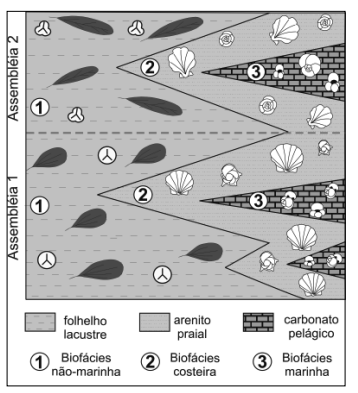
\includegraphics[width=0.6\linewidth]{bioestratigrafia.png}
    \caption{Uso de fósseis na correlação de estratos separados espacialmente.}
\end{figure}
\cite{zerfass2008foraminiferos}

\subsection{Interações Ecológicas}


\begin{definicao}
\textbf{Interações ecológicas}: São as relações estabelecidas entre organismos de uma mesma espécie ou de espécies diferentes, bem como entre esses organismos e o ambiente em que vivem. Essas interações influenciam a distribuição, a abundância e a dinâmica das populações ao longo do tempo.
\end{definicao}

As interações ecológicas podem ser classificadas em dois grandes grupos:

\begin{itemize}
    \item \textbf{Interações intraespecíficas}: ocorrem entre indivíduos da mesma espécie, podendo envolver cooperação (como sociedades e colônias) ou competição por recursos.

    \item \textbf{Interações interespecíficas}: ocorrem entre indivíduos de espécies diferentes, incluindo relações como predação, competição, mutualismo, comensalismo e parasitismo.
\end{itemize}

Essas interações constituem um dos fundamentos da ecologia, pois determinam o fluxo de energia, a ciclagem de nutrientes e a estrutura das comunidades biológicas. Em escala geológica, as interações ecológicas também se refletem no registro fossilífero, permitindo inferir relações entre organismos e ambientes do passado.

As interações ecológicas possuem relação direta com a geologia moderna, na medida em que os organismos não apenas habitam os ambientes geológicos, mas também os modificam e deixam registros de sua atividade. No registro fossilífero, essas interações se manifestam por meio de associações de organismos, estruturas biogênicas e padrões de sucessão faunística. Além disso, a atividade biológica influencia processos sedimentares, contribuindo para a formação de depósitos específicos, como recifes carbonáticos e sedimentos bioturbados. Dessa forma, a interpretação geológica contemporânea incorpora não apenas os aspectos físicos e químicos das rochas, mas também as relações ecológicas que condicionaram sua formação, permitindo uma reconstrução mais completa dos ambientes do passado.

Na geologia moderna, as interações ecológicas assumem especial importância no estudo das bacias sedimentares, uma vez que estas representam os principais sítios de deposição, preservação fossilífera e registro da evolução ambiental. Em uma bacia sedimentar, os organismos participam ativamente dos processos geológicos, influenciando a produção, retrabalhamento e modificação dos sedimentos. Estruturas como recifes, níveis ricos em matéria orgânica e feições de bioturbação mostram que a sedimentação não resulta apenas de processos físicos e químicos, mas também da ação dos seres vivos e de suas relações ecológicas. Assim, o estudo das bacias sedimentares na geologia contemporânea requer uma abordagem integrada, na qual a dinâmica deposicional, a paleoecologia e a sucessão estratigráfica sejam interpretadas de forma conjunta.

Assim, as bacias sedimentares constituem o espaço privilegiado em que a interação entre processos geológicos e ecológicos se torna registrada e preservada no tempo geológico.

\section{Estruturas tectônicas e halocinese}

As estruturas tectônicas modificam a geometria das camadas e, por isso, influenciam a leitura do registro estratigráfico, a geração de relevo e a organização das bacias.

\subsection{Dobras}
\begin{definicao}

Os dobramentos \textbf{sinclinais} são estruturas geológicas em que as camadas rochosas se curvam de modo côncavo para cima, formando uma dobra cuja parte central contém, em geral, as camadas mais recentes. Em um sinclinal, os flancos mergulham em direção ao eixo da dobra.

\end{definicao}

\subsection{Falhas}

Uma \textbf{falha} é uma descontinuidade ao longo da qual ocorreu deslocamento relativo entre blocos rochosos. A classificação cinemática considera a direção do movimento:

\begin{itemize}
  \item \textbf{falha normal}: o bloco de teto desce em relação ao bloco de muro; associa-se principalmente à extensão;
  \item \textbf{falha reversa}: o bloco de teto sobe em relação ao bloco de muro; associa-se principalmente à compressão;
  \item \textbf{falha transcorrente}: o deslocamento predominante é horizontal e pode ser dextral ou sinistral;
  \item \textbf{falha oblíqua}: combina componentes vertical e horizontal importantes.
\end{itemize}

Falhas lístricas possuem superfície curva, geralmente com diminuição do mergulho em profundidade. Em bacias extensionais, falhas normais podem delimitar grábens e semigrábens. Quando o deslocamento ocorre simultaneamente à deposição e produz variação sistemática da espessura dos estratos, usa-se o termo \textbf{falha de crescimento} \parencite{fossen2016}.

\subsection{Exemplo: Bacia do Recôncavo}

A Bacia do Recôncavo integra o sistema rifte Recôncavo--Tucano--Jatobá, desenvolvido durante a ruptura continental relacionada à abertura do Atlântico Sul. Seu arcabouço apresenta blocos assimétricos controlados predominantemente por falhas normais. A Falha de Salvador limita a bacia a leste, enquanto a Falha de Maragogipe integra seu limite ocidental. O preenchimento registra sistemas continentais, especialmente lacustres, fluviais e deltaicos \parencite{anp_reconcavo,magnavita2005}.

Esse exemplo mostra a relação entre:

\[
\begin{gathered}
\text{extensão crustal}
\rightarrow
\text{falhamento normal}
\rightarrow
\text{subsidência}
\\[-0.2em]
\rightarrow
\text{criação de acomodação}
\rightarrow
\text{preenchimento sedimentar}.
\end{gathered}
\]

\subsection{Exemplo: estruturas do estado do Rio de Janeiro}

O mapa geológico estadual registra estruturas de diferentes naturezas e idades, incluindo falhas, zonas de cisalhamento e lineamentos que afetam o embasamento e as coberturas sedimentares. Sua interpretação exige distinguir estruturas antigas do Cinturão Ribeira de reativações posteriores relacionadas à evolução da margem continental e do relevo do Sudeste. Assim, uma direção cartográfica semelhante não prova, por si só, que duas falhas tenham a mesma idade ou cinemática \parencite{heilbron2016,fossen2016}.

\begin{definicao}
 Os dobramentos \textbf{anticlinais} são estruturas geológicas em que as camadas rochosas se curvam de modo convexo para cima, formando uma dobra cuja parte central contém, em geral, as camadas mais antigas. Em um anticlinal, os flancos mergulham em sentido oposto ao eixo da dobra.   
\end{definicao}

\subsection{Diápiros e estruturas salinas}

\begin{definicao}
Os \textbf{diápiros} são estruturas geológicas formadas pela ascensão de materiais mais dúcteis e menos densos através de camadas rochosas superiores mais rígidas e mais densas. Essa ascensão ocorre em razão da diferença de densidade entre os materiais e da capacidade de deformação plástica da massa ascendente.

Os \textbf{diápiros de sal} são diápiros constituídos predominantemente por evaporitos, especialmente halita, podendo também incluir anidrita, gipsita e outros sais. Em profundidade, o sal comporta-se de maneira dúctil e, por ser menos denso que grande parte das rochas sedimentares que o recobrem, tende a migrar para níveis superiores, deformando as camadas encaixantes.

Os diápiros de sal ocorrem em \textbf{bacias sedimentares evaporíticas}, isto é, em bacias nas quais houve deposição de espessas camadas de sal em ambientes de intensa evaporação. Sua formação inicia-se com a deposição desses evaporitos, seguida pelo soterramento por sedimentos mais densos. Com o aumento da sobrecarga, o sal passa a fluir lentamente devido ao seu comportamento plástico e à diferença de densidade, podendo ascender e formar estruturas como domos e muralhas salinas. Essas estruturas são comuns em regiões como o Golfo do México, o Mar do Norte, o Oriente Médio e a margem continental brasileira, especialmente em áreas associadas ao pré-sal \parencite{jacksonhudec2017}.

\end{definicao}

\section{Fácies, associações de fácies e ambientes deposicionais}

\begin{definicao}
Uma \textbf{fácies sedimentar} é um corpo de sedimento ou rocha caracterizado por um
conjunto de propriedades observáveis que o distingue dos corpos adjacentes. Essas
propriedades podem incluir litologia, granulometria, estruturas sedimentares, fósseis,
cor, geometria e contatos.
\end{definicao}

A descrição de uma fácies deve preceder sua interpretação. Por exemplo, ``arenito fino
com laminação cruzada e bioturbação esparsa'' é uma descrição; ``depósito de canal de
maré'' é uma interpretação que precisa ser sustentada pelo conjunto de evidências.

\subsection{Códigos de litofácies}

Os códigos de litofácies combinam uma letra maiúscula que indica a classe granulométrica
com letras minúsculas que representam estruturas ou características. Em esquemas
derivados de Miall, por exemplo, \emph{G} indica cascalho, \emph{S} indica areia e
\emph{F} indica sedimentos finos. O significado completo de cada código deve ser
declarado no trabalho, porque há adaptações entre autores e ambientes
\parencite{miall1978,nichols2009}.

\subsection{Associação de fácies}

Uma fácies isolada raramente define um ambiente deposicional de maneira inequívoca. Uma
\textbf{associação de fácies} reúne fácies que ocorrem repetidamente juntas e que podem
ser relacionadas por processos sedimentares compatíveis. A interpretação ganha força
quando considera:

\begin{itemize}
  \item a sucessão vertical das fácies;
  \item as relações laterais;
  \item a geometria dos corpos;
  \item as superfícies erosivas ou de reativação;
  \item a direção das paleocorrentes;
  \item os fósseis e icnofósseis;
  \item o contexto estratigráfico regional.
\end{itemize}

\subsection{Sucessão de fácies}

Uma \textbf{sucessão de fácies} é a ordem vertical ou lateral em que diferentes fácies
aparecem. Tendências granodecrescentes podem registrar diminuição da energia do fluxo,
como em certos preenchimentos de canal. Tendências granocrescentes podem acompanhar a
progradação de sistemas deposicionais. Essas interpretações, entretanto, dependem da
geometria, das superfícies limitantes e do ambiente analisado.

\subsection{Ambientes continentais, transicionais e marinhos}

Em escala ampla, os ambientes deposicionais podem ser agrupados em:

\begin{itemize}
  \item \textbf{continentais}: fluviais, lacustres, eólicos, glaciais e leques aluviais;
  \item \textbf{transicionais}: deltas, estuários, planícies de maré e sistemas costeiros;
  \item \textbf{marinhos}: plataforma, talude, bacia profunda, recifes e outros sistemas
        oceânicos.
\end{itemize}

Estratificação espinha de peixe, superfícies de reativação e alternância de laminações de
areia e lama podem indicar reversão periódica de correntes, comum em ambientes de maré.
Camadas com estratificação cruzada hummocky são associadas a fluxos combinados gerados
por tempestades em ambientes marinhos rasos. Nenhuma dessas feições deve ser usada
isoladamente como diagnóstico definitivo \parencite{harms1975,nichols2009}.

\section{Guia de estudos}

\subsection{Como estudar esta matéria}

Em vez de memorizar listas isoladas, acompanhe o caminho do material sedimentar:

\[
\boxed{
\begin{gathered}
\text{rocha-fonte}
\rightarrow
\text{intemperismo}
\rightarrow
\text{erosão e transporte}
\\
\rightarrow
\text{deposição}
\rightarrow
\text{diagênese}
\rightarrow
\text{rocha sedimentar}
\end{gathered}
}
\]

Para cada etapa, procure responder: \emph{qual é o processo, qual é o agente, qual
produto é gerado e que evidência fica preservada?}

\subsection{Resumo dos processos}

\begin{table}[H]
  \centering
  \caption{Relações fundamentais do sistema sedimentar.}
  \begin{tabularx}{\textwidth}{>{\bfseries}lXX}
    \toprule
    Etapa & Processo principal & Produto ou registro \\
    \midrule
    Intemperismo & Desagregação e decomposição da rocha & Clastos, argilominerais e íons dissolvidos \\
    Erosão & Remoção do material da área-fonte & Disponibilização de sedimento \\
    Transporte & Tração, saltação, suspensão e solução & Seleção, abrasão e orientação \\
    Deposição & Perda de competência/capacidade ou precipitação & Camadas e formas de leito \\
    Diagênese & Compactação, cimentação e reações pós-deposicionais & Litificação e modificação dos poros \\
    \bottomrule
  \end{tabularx}
\end{table}

\subsection{Distinções que não devem ser confundidas}

\begin{table}[H]
  \centering
  \caption{Conceitos próximos, mas diferentes.}
  \begin{tabularx}{\textwidth}{>{\bfseries}lXX}
    \toprule
    Par & Primeiro conceito & Segundo conceito \\
    \midrule
    Intemperismo/erosão & Altera a rocha no local & Remove o material \\
    Competência/capacidade & Maior tamanho transportável & Quantidade total transportável \\
    Arredondamento/esfericidade & Curvatura de arestas e vértices & Aproximação da forma a uma esfera \\
    Matriz/cimento & Material detrítico fino & Precipitado diagenético \\
    Porosidade/permeabilidade & Volume de vazios & Conectividade para o fluxo \\
    Bacia de sedimentação/bacia sedimentar & Local atual de deposição & Unidade geológica subsidente e preenchida \\
    Fácies/ambiente & Conjunto observável de características & Interpretação genética \\
    \bottomrule
  \end{tabularx}
\end{table}

\subsection{Equações e limites essenciais}

\begin{align*}
  \phi &= -\log_2 d_{\mathrm{mm}}, \\
  \mathrm{Fr} &= \frac{U}{\sqrt{gD}}.
\end{align*}

Interpretação do número de Froude:

\[
\mathrm{Fr}<1\;\text{subcrítico},
\qquad
\mathrm{Fr}=1\;\text{crítico},
\qquad
\mathrm{Fr}>1\;\text{supercrítico}.
\]

Limites granulométricos:

\[
\begin{array}{rcl}
d>\SI{2}{\milli\metre} &:& \text{cascalho},\\
\SI{0.0625}{\milli\metre}\le d\le\SI{2}{\milli\metre} &:& \text{areia},\\
\SI{0.0039}{\milli\metre}\le d<\SI{0.0625}{\milli\metre} &:& \text{silte},\\
d<\SI{0.0039}{\milli\metre} &:& \text{argila}.
\end{array}
\]

\subsection{Roteiro para descrever uma amostra siliciclástica}

Siga sempre a mesma sequência:

\begin{enumerate}
  \item determine a classe granulométrica dominante;
  \item estime a distribuição das frações cascalho, areia e lama;
  \item descreva o grau de seleção;
  \item descreva arredondamento e esfericidade separadamente;
  \item reconheça arcabouço, matriz, cimento e poros;
  \item identifique quartzo, feldspatos e fragmentos líticos;
  \item observe cor, estruturas e fósseis;
  \item atribua o nome da rocha;
  \item somente depois proponha processos e ambiente deposicional.
\end{enumerate}

\subsection{Classificação rápida das rochas siliciclásticas}

\begin{table}[H]
  \centering
  \caption{Critérios principais de classificação.}
  \begin{tabularx}{\textwidth}{>{\bfseries}lXX}
    \toprule
    Grupo & Critério principal & Subdivisões úteis \\
    \midrule
    Conglomerados & Clastos maiores que \SI{2}{\milli\metre} & Clasto/matriz-suportado; mono/oligo/polimítico \\
    Arenitos & Areia e composição Q--F--L & Arenita ou wacke; quartzosa, feldspática ou lítica \\
    Pelitos & Silte, argila e fissilidade & Siltito, argilito, lamito e folhelho \\
    \bottomrule
  \end{tabularx}
\end{table}

\subsection{Estruturas sedimentares e interpretação}

\begin{table}[H]
  \centering
  \caption{Estruturas e informações que podem fornecer.}
  \begin{tabularx}{\textwidth}{>{\bfseries}lX}
    \toprule
    Estrutura & Interpretação possível \\
    \midrule
    Estratificação cruzada & Migração de formas de leito e paleocorrente \\
    Ripple assimétrico & Corrente predominantemente unidirecional \\
    Ripple simétrico & Movimento oscilatório por ondas \\
    Gradação normal & Redução da energia durante a deposição \\
    Gretas de dessecação & Exposição subaérea e perda de água \\
    Marcas de sola & Erosão do substrato e possível sentido de fluxo \\
    Flaser/wavy/lenticular & Alternância de transporte de areia e decantação de lama \\
    Hummocky/swaley & Fluxo combinado relacionado a tempestades \\
    Imbricação & Orientação de clastos e possível paleocorrente \\
    Bioturbação & Atividade de organismos no substrato \\
    Estruturas de carga/escape & Instabilidade e movimentação de sedimento saturado \\
    \bottomrule
  \end{tabularx}
\end{table}

Uma estrutura isolada raramente determina um ambiente. A interpretação deve combinar
litologia, granulometria, geometria, contatos, paleocorrentes, fósseis e associação de
fácies.

\subsection{Perguntas de revisão}

\begin{enumerate}
  \item Qual é a diferença entre intemperismo físico e químico?
  \item Por que a água é importante no intemperismo químico?
  \item Que relação geral existe entre as séries de Bowen e Goldich?
  \item Diferencie erosão, transporte e deposição.
  \item Diferencie competência e capacidade de um fluxo.
  \item Quais são os quatro modos fundamentais de transporte sedimentar?
  \item Por que argilas exigem maior velocidade para serem erodidas do que alguns grãos de areia?
  \item O que significam \(\mathrm{Fr}<1\) e \(\mathrm{Fr}>1\)?
  \item Diferencie seleção, arredondamento e esfericidade.
  \item Quais são os limites fundamentais de cascalho, areia, silte e argila?
  \item Diferencie conglomerado clasto-suportado e matriz-suportado.
  \item Qual é a diferença entre arenita e wacke?
  \item O que representam os polos Q, F e L?
  \item Diferencie matriz e cimento.
  \item Quais processos fazem parte da diagênese?
  \item Como distinguir ripple de corrente e ripple de onda?
  \item O que uma estratificação espinha de peixe pode indicar?
  \item Por que fácies e ambiente deposicional não são sinônimos?
  \item Como soerguimento e subsidência participam do sistema sedimentar?
  \item O que uma discordância representa no registro geológico?
\end{enumerate}

\subsection{Respostas resumidas}

\begin{enumerate}
  \item O físico desagrega sem mudança mineralógica dominante; o químico transforma ou dissolve minerais.
  \item Ela atua como solvente, reagente e meio de transporte de íons.
  \item Minerais que cristalizam em temperaturas mais altas tendem a ser menos estáveis na superfície.
  \item Erosão remove, transporte desloca e deposição acumula.
  \item Competência refere-se ao tamanho máximo; capacidade, à quantidade total.
  \item Tração, saltação, suspensão e solução.
  \item Devido à coesão eletroquímica entre partículas finas.
  \item Fluxo subcrítico e supercrítico, respectivamente.
  \item Dispersão de tamanhos; curvatura das arestas; forma global.
  \item \SI{2}{\milli\metre}, \SI{0.0625}{\milli\metre} e \SI{0.0039}{\milli\metre}.
  \item No primeiro os clastos se tocam; no segundo ficam dispersos na matriz.
  \item A diferença principal é a proporção de matriz fina.
  \item Quartzo, feldspatos e fragmentos líticos.
  \item Matriz é detrítica; cimento é precipitado durante a diagênese.
  \item Compactação, cimentação, dissolução, recristalização e substituição.
  \item O de corrente tende a ser assimétrico; o de onda tende a ser simétrico.
  \item Reversão periódica das correntes, comum em sistemas de maré.
  \item Fácies é descrição; ambiente é interpretação.
  \item Soerguimento favorece exposição e erosão; subsidência cria acomodação.
  \item Um intervalo de não deposição e/ou erosão, isto é, tempo ausente.
\end{enumerate}


\printbibliography[heading=bibintoc,title={Referências}]

\appendix
\section{Carta cronoestratigráfica}
\begin{landscape}
  \centering
  \includegraphics[width=\linewidth,height=0.92\textheight,keepaspectratio]
    {ChronostratChart2023-04BRPortuguese.pdf}
\end{landscape}

\section{Escala granulométrica de Wentworth}
\begin{figure}[H]
  \centering
  \includegraphics[width=0.9\linewidth]
    {M1U5-Table5.5. The Wentworth scale.pdf}
  \caption{Escala granulométrica de Wentworth.}
\end{figure}

\end{document}
